\documentclass[11pt,a4paper]{report}

% ------------------------- Encodage et langue -------------------------
\usepackage[T1]{fontenc}
\usepackage[utf8]{inputenc}
\usepackage[french]{babel}
\usepackage{lmodern}

% ------------------------- Mise en page -------------------------------
\usepackage[margin=2.5cm]{geometry}
\usepackage{setspace}
\onehalfspacing
\usepackage{parskip}

% ------------------------- Figures et tableaux ------------------------
\usepackage{graphicx}
\graphicspath{{report_plots/}{./}}
\usepackage{float}
\usepackage{booktabs}
\usepackage{longtable}
\usepackage{array}
\usepackage{calc}
\usepackage{etoolbox}

% ------------------------- Mathématiques ------------------------------
\usepackage{amsmath}
\usepackage{amssymb}

% ------------------------- Liens et méta ------------------------------
\usepackage[hidelinks]{hyperref}
\hypersetup{
  pdftitle={Classification d'images de félins par des modèles d'apprentissage implémentés from scratch en Rust},
  pdfauthor={Léo Croft, Eric Sang},
  pdflang={fr}
}

% Compatibilité avec la sortie pandoc
\providecommand{\tightlist}{\setlength{\itemsep}{0pt}\setlength{\parskip}{0pt}}
\makeatletter
\providecommand{\pandocbounded}[1]{#1}
\makeatother
\newcolumntype{L}[1]{>{\raggedright\arraybackslash}p{#1}}

% ------------------------- En-têtes -----------------------------------
\usepackage{fancyhdr}
\pagestyle{fancy}
\fancyhf{}
\fancyhead[L]{\small\leftmark}
\fancyfoot[C]{\thepage}
\renewcommand{\headrulewidth}{0.4pt}

\begin{document}

% ============================ PAGE DE TITRE ============================
\begin{titlepage}
  \centering
  \vspace*{2cm}
  {\LARGE \textbf{Projet Annuel}\par}
  \vspace{1cm}
  {\Huge \bfseries Classification d'images de félins par des modèles d'apprentissage implémentés \emph{from scratch} en Rust\par}
  \vspace{1.5cm}
  {\Large \texttt{felidae\_classifier} --- Classification chat / lion / guépard\par}
  \vfill
  {\Large Léo Croft \& Eric Sang\par}
  \vspace{0.3cm}
  {\large ESGI --- 3IABD2\par}
  \vspace{1.5cm}
\end{titlepage}

% ============================ TABLE DES MATIÈRES =======================
\tableofcontents
\clearpage

% ============================ CORPS DU RAPPORT =========================
\hypertarget{introduction-et-objectifs-du-projet}{%
\chapter{Introduction et objectifs du
projet}\label{introduction-et-objectifs-du-projet}}

Ce projet annuel a pour objectif la conception, l'implémentation et
l'étude expérimentale d'une chaîne complète de classification d'images,
construite intégralement from scratch. Le problème retenu consiste à
distinguer trois espèces de félins visuellement proches : le chat
domestique, le lion et le guépard. Ce choix n'est pas anodin. Les trois
classes partagent des couleurs de pelage, des morphologies et des
contextes de prise de vue similaires, ce qui rend le problème
suffisamment difficile pour révéler les forces et les limites de chaque
famille de modèles, tout en restant traitable avec des moyens
raisonnables.

Conformément au sujet, quatre modèles ont été implémentés sans recours à
une bibliothèque d'apprentissage automatique : le modèle linéaire de
Rosenblatt, le Perceptron Multi-Couches, le réseau à fonctions de base
radiales et le Support Vector Machine. L'ensemble est écrit en Rust sous
la forme d'une bibliothèque dynamique, exposée au monde Python par une
interface C, ce qui permet à la fois des exécutables de test natifs, des
scripts d'expérimentation Python et une interface graphique interactive.
Chaque ligne de code du projet peut être expliquée et défendue,
condition que le sujet érige en exigence première.

Au-delà de la performance brute, notre démarche a consisté à reproduire
sur nos propres modèles et nos propres données les phénomènes
fondamentaux étudiés en cours : le compromis entre sous-apprentissage et
sur-apprentissage, l'influence du nombre de paramètres sur la
généralisation, le rôle de la représentation d'entrée, et la différence
essentielle entre minimiser l'erreur sur les exemples et généraliser. Ce
rapport présente le jeu de données, l'architecture logicielle, l'étude
expérimentale de chaque modèle, une comparaison transversale, puis un
chapitre dédié aux difficultés rencontrées au fil du projet et à la
manière dont nous les avons résolues.

\begin{center}\rule{0.5\linewidth}{0.5pt}\end{center}

\hypertarget{constitution-et-nettoyage-du-jeu-de-donnuxe9es}{%
\chapter{Constitution et nettoyage du jeu de
données}\label{constitution-et-nettoyage-du-jeu-de-donnuxe9es}}

\hypertarget{collecte}{%
\section{Collecte}\label{collecte}}

Le jeu de données brut regroupe environ trente mille images réparties
entre les trois classes, rassemblées à partir de sources publiques.
Comme toujours avec des images collectées en masse, la qualité initiale
était très hétérogène : de nombreuses images contenaient l'animal en
tout petit dans un décor dominant, plusieurs animaux à la fois, ou pas
d'animal du tout, et certaines étaient dans des formats ou des modes de
couleur exotiques.

\hypertarget{nettoyage-par-duxe9tection-dobjets}{%
\section{Nettoyage par détection
d'objets}\label{nettoyage-par-duxe9tection-dobjets}}

Plutôt que de trier trente mille images à la main, nous avons automatisé
le nettoyage à l'aide d'un détecteur d'objets pré-entraîné, YOLOv8,
utilisé uniquement comme outil de préparation de données et jamais comme
composant de nos classifieurs. Le script de nettoyage parcourt chaque
image, détecte la boîte englobante de l'animal, recadre l'image sur
cette boîte, et rejette les images sans animal détecté ainsi que celles
dont la détection est trop petite pour contenir une information
exploitable. Ce recadrage a un double effet bénéfique : il centre
l'information utile, l'animal lui-même, et il élimine une grande partie
du décor qui, sinon, parasiterait les caractéristiques de couleur et de
texture calculées ensuite.

Un problème concret est apparu pendant ce nettoyage : certaines images
JPEG étaient en mode palette, un mode de couleur indexé que la
bibliothèque d'imagerie refuse de réenregistrer en JPEG. La solution a
consisté à convertir systématiquement chaque image en RGB avant
sauvegarde. À l'issue du nettoyage, environ vingt-six mille images
exploitables ont été conservées, organisées en trois sous-dossiers, un
par classe, la structure de dossiers faisant office d'étiquetage.

\hypertarget{chargement-et-mise-en-cache}{%
\section{Chargement et mise en
cache}\label{chargement-et-mise-en-cache}}

Le chargement des images et l'extraction des caractéristiques étant
coûteux à répéter, la bibliothèque construit le jeu de données une seule
fois puis le sérialise dans un fichier binaire de cache. Les exécutions
suivantes rechargent directement ce cache, ce qui réduit le temps de
démarrage des expériences de plusieurs minutes à quelques secondes. Le
nom du fichier de cache encode la représentation et la taille demandées,
si bien que les différentes configurations coexistent sans risque de
charger des caractéristiques de mauvaise dimension.

\begin{center}\rule{0.5\linewidth}{0.5pt}\end{center}

\hypertarget{architecture-logicielle-de-la-bibliothuxe8que}{%
\chapter{Architecture logicielle de la
bibliothèque}\label{architecture-logicielle-de-la-bibliothuxe8que}}

\hypertarget{une-bibliothuxe8que-rust-from-scratch}{%
\section{Une bibliothèque Rust from
scratch}\label{une-bibliothuxe8que-rust-from-scratch}}

Le cœur du projet est une bibliothèque Rust, felidae\_classifier,
compilée en bibliothèque dynamique. Le module tensor fournit le type
Matrix, une matrice de flottants en mémoire contiguë ligne par ligne,
avec les opérations nécessaires aux modèles : produit matriciel,
transposée, et inversion par élimination de Gauss-Jordan sur matrice
augmentée. Toute l'algèbre linéaire du projet repose sur ce seul type,
sans dépendance externe de calcul numérique.

Le module data définit la structure Dataset, son enregistrement et son
chargement binaires, la construction depuis l'arborescence d'images,
l'encodage un-parmi-n des étiquettes en valeurs plus un et moins un
adaptées à la tangente hyperbolique, et le découpage apprentissage-test.
Ce découpage est stratifié : les indices sont regroupés par classe,
chaque classe est mélangée avec une graine qui lui est propre, dérivée
de la graine globale par une multiplication par un grand nombre impair
afin d'éviter toute collision entre graines voisines, puis chaque classe
contribue la même proportion au jeu de test. La même graine produit
toujours le même découpage, ce qui rend toutes nos expériences
reproductibles.

Le module features regroupe les deux représentations d'entrée décrites
au chapitre suivant ainsi qu'un StandardScaler qui centre et réduit
chaque caractéristique, ses statistiques étant apprises sur le seul jeu
d'apprentissage puis appliquées au jeu de test. Le module models
contient les quatre modèles, chacun dans son sous-module, et le module
ffi expose l'ensemble au monde extérieur par des fonctions C.

\hypertarget{qualituxe9-et-tests}{%
\section{Qualité et tests}\label{qualituxe9-et-tests}}

La bibliothèque est couverte par plus de cent tests unitaires, exécutés
à chaque modification. Ces tests se sont révélés être bien davantage
qu'une formalité : à plusieurs reprises, ils ont détecté des erreurs
réelles avant qu'elles n'atteignent les expériences, dont un bug
d'accumulation dans le calcul de distance euclidienne que nous
détaillons au chapitre des difficultés. Les tests couvrent les
opérations matricielles, le découpage stratifié, chaque modèle sur des
jeux synthétiques minuscules aux résultats vérifiables à la main, et les
cycles complets de sauvegarde puis rechargement de chaque modèle.

\hypertarget{interopuxe9rabilituxe9-et-applications}{%
\section{Interopérabilité et
applications}\label{interopuxe9rabilituxe9-et-applications}}

Trois consommateurs utilisent la bibliothèque. Deux exécutables Rust,
test\_synthetic et test\_real, déroulent respectivement les cas de tests
synthétiques sur les quatre modèles et l'entraînement complet sur le
vrai jeu de données, avec matrices de confusion et sauvegarde des
modèles. Des scripts Python d'expérimentation appellent la bibliothèque
via cffi pour produire toutes les figures de ce rapport. Enfin, une
interface graphique Gradio permet d'entraîner chaque modèle avec ses
hyperparamètres, de classifier une image téléversée par le modèle de son
choix, et de consulter l'état des modèles sauvegardés. L'entraînement du
MLP journalise en outre la perte et les précisions dans TensorBoard à
chaque époque, ce qui a servi de base aux courbes d'apprentissage du
rapport.

Chaque modèle sauvegardé s'accompagne d'un fichier de métadonnées
indiquant la représentation d'entrée avec laquelle il a été entraîné et
ses hyperparamètres, de sorte que l'inférence reproduit exactement le
prétraitement de l'entraînement. Les formats binaires de sauvegarde
suivent tous le même schéma : un nombre magique identifiant le type de
modèle, une version de format, puis les dimensions et les données, ce
qui permet de détecter immédiatement le chargement d'un fichier du
mauvais type.

\begin{center}\rule{0.5\linewidth}{0.5pt}\end{center}

\hypertarget{repruxe9sentations-dentruxe9e-et-contrainte-de-dimensionnement}{%
\chapter{Représentations d'entrée et contrainte de
dimensionnement}\label{repruxe9sentations-dentruxe9e-et-contrainte-de-dimensionnement}}

Deux représentations d'entrée coexistent dans tout le projet et sont
comparées à plusieurs reprises.

La première, dite extract, réduit chaque image recadrée en trente-deux
par trente-deux pixels puis en tire vingt caractéristiques : la moyenne
et l'écart-type de chacun des trois canaux de couleur, soit six valeurs,
un histogramme de luminosité à huit intervalles, et six mesures de
densité de contours à deux seuils. Cette représentation compacte
respecte la contrainte que nous nous sommes fixée, inspirée de la règle
de dimensionnement du cours, de ne jamais dépasser un nombre de
caractéristiques supérieur à dix pour cent de la taille du jeu
d'apprentissage.

La seconde, dite flatten, aplatit directement les pixels bruts de
l'image trente-deux par trente-deux en couleur, soit trois mille
soixante-douze valeurs par exemple. Cette représentation transporte
davantage d'information brute mais viole la contrainte des dix pour cent
dès que le jeu d'apprentissage descend sous trente mille exemples, et
nous verrons qu'elle met les méthodes à noyau en grande difficulté. La
confrontation systématique de ces deux représentations, modèle par
modèle, constitue l'un des fils conducteurs de ce rapport : elle
montrera que le choix de la représentation ne déplace pas seulement la
précision globale de quelques points, mais change la nature même des
erreurs commises.

\begin{center}\rule{0.5\linewidth}{0.5pt}\end{center}

\hypertarget{uxe9tude-expuxe9rimentale-du-perceptron-de-rosenblatt}{%
\chapter{Étude expérimentale du Perceptron de
Rosenblatt}\label{uxe9tude-expuxe9rimentale-du-perceptron-de-rosenblatt}}

\begin{center}\rule{0.5\linewidth}{0.5pt}\end{center}

\hypertarget{cadre-muxe9thodologique}{%
\section{Cadre méthodologique}\label{cadre-muxe9thodologique}}

Le perceptron de Rosenblatt est le modèle linéaire le plus élémentaire
de notre projet. Contrairement au MLP qui empile des couches de neurones
avec des fonctions d'activation non linéaires, le perceptron ne dispose
que d'une seule couche de poids directement connectée aux entrées, sans
transformation intermédiaire. La frontière de décision qu'il trace dans
l'espace des caractéristiques est donc un hyperplan, ce qui le rend
incapable de résoudre des problèmes non linéairement séparables. Pour
gérer notre problème à trois classes, nous utilisons une architecture «
un contre tous » composée de trois perceptrons indépendants, un pour
chaque classe (chat, lion, guépard), chacun apprenant à distinguer sa
classe de toutes les autres.

Les résultats présentés ici utilisent la représentation par
caractéristiques extraites, un vecteur de vingt dimensions regroupant
des statistiques de couleur, un histogramme de luminosité et des mesures
de densité de contours. Ce choix de représentation compacte, plutôt
qu'un aplatissement brut des pixels, respecte la contrainte que nous
nous sommes fixée de ne jamais dépasser un nombre de caractéristiques
supérieur à dix pour cent de la taille du jeu d'apprentissage.

Toutes les expériences qui suivent isolent un seul paramètre à la fois,
de manière à mettre en évidence son influence propre sur la vitesse de
convergence et sur la capacité de généralisation du modèle. Sauf mention
contraire, nous utilisons un taux d'apprentissage de 0,01, cinq cents
époques et une graine aléatoire fixée. Le découpage entre apprentissage
et test suit une répartition de quatre-vingts pour cent contre vingt
pour cent.

\begin{center}\rule{0.5\linewidth}{0.5pt}\end{center}

\hypertarget{expuxe9rience-1-influence-du-taux-dapprentissage}{%
\section{Expérience 1 --- Influence du taux
d'apprentissage}\label{expuxe9rience-1-influence-du-taux-dapprentissage}}

Nous avons fait varier le taux d'apprentissage sur six valeurs allant de
0,0001 à 0,5 en maintenant le nombre d'époques fixé à cinq cents. La
courbe obtenue présente un pic net à 0,01, avec environ quarante-sept
pour cent en apprentissage et quarante-six pour cent en test, précédé
d'une montée régulière depuis 0,0001. Juste après ce pic, la précision
s'effondre brutalement autour de 0,05, retombant à environ trente-sept
pour cent en apprentissage et trente-sept pour cent en test, avant de
remonter partiellement à 0,1 et de se stabiliser autour de
quarante-quatre pour cent jusqu'à 0,5.

Ce creux étroit juste après le taux optimal est caractéristique du
perceptron simple et s'explique par l'absence de fonction d'activation
continue. Contrairement au MLP où un taux trop élevé fait simplement
diverger une descente de gradient lisse, le perceptron met à jour ses
poids uniquement sur les exemples mal classés, avec des sauts discrets
proportionnels au taux d'apprentissage. Au voisinage immédiat du taux
optimal, ces sauts deviennent juste assez grands pour faire osciller les
poids autour de la frontière au lieu de la stabiliser, ce qui explique
l'effondrement localisé à 0,05. La remontée partielle au-delà suggère
que le modèle retrouve ensuite une forme de stabilité, différente de la
solution optimale mais moins chaotique que le creux qui la précède.

\begin{figure}[htbp]
\centering
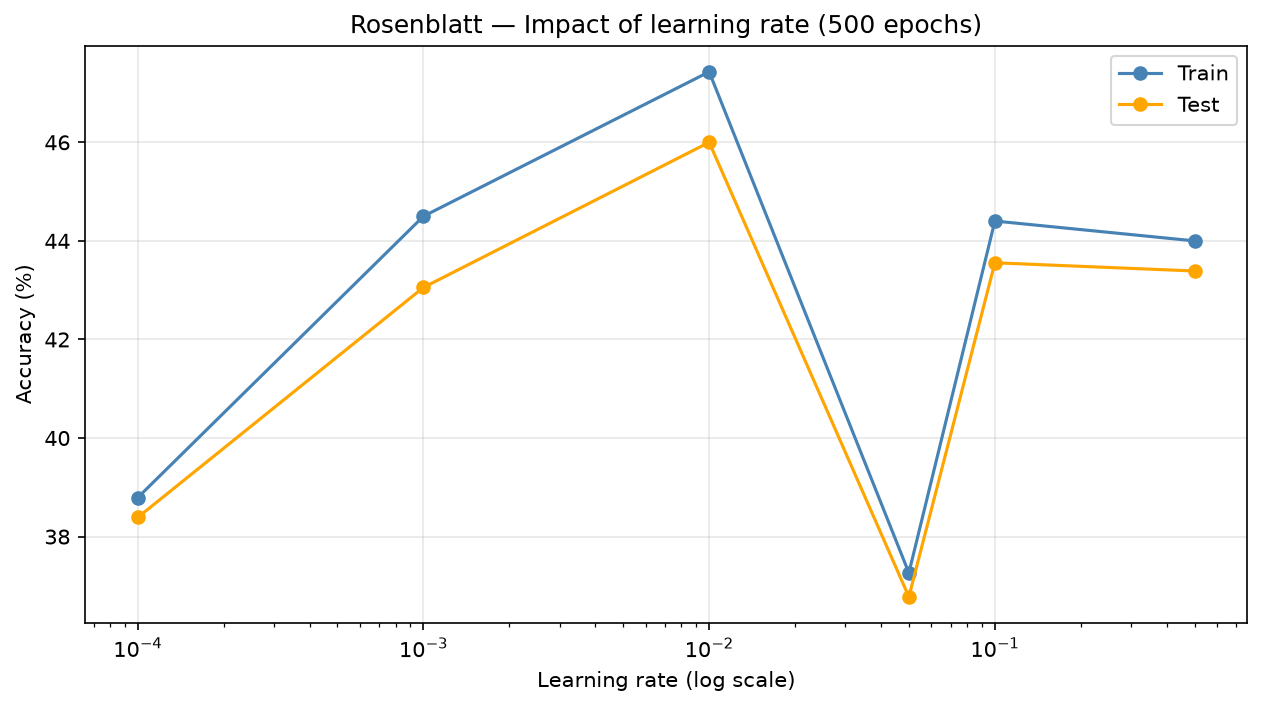
\includegraphics[width=0.85\linewidth]{report_plots/rosenblatt_lr_sweep.png}
\caption{Rosenblatt --- Influence du taux d'apprentissage}
\end{figure}

\begin{center}\rule{0.5\linewidth}{0.5pt}\end{center}

\hypertarget{expuxe9rience-2-influence-du-nombre-duxe9poques}{%
\section{Expérience 2 --- Influence du nombre
d'époques}\label{expuxe9rience-2-influence-du-nombre-duxe9poques}}

Nous avons ensuite observé l'évolution des précisions en fonction du
nombre d'époques, de dix à cinq mille, à un taux d'apprentissage fixé à
0,01, la valeur optimale identifiée par l'expérience précédente. La
courbe n'est pas monotone : elle progresse d'abord de dix à cent
époques, autour de trente-huit à quarante-quatre pour cent, redescend
légèrement à deux cent cinquante époques, remonte à un premier sommet
local à cinq cents époques avec environ quarante-sept pour cent en
apprentissage et quarante-six pour cent en test, puis retombe à mille
époques autour de quarante-quatre et quarante-trois pour cent.

Le résultat le plus notable apparaît au-delà de mille époques : plutôt
que de se dégrader, la précision reprend une progression nette et
atteint son maximum absolu à cinq mille époques, avec environ
cinquante-trois pour cent en apprentissage et cinquante-deux pour cent
en test. Les deux courbes restent proches l'une de l'autre tout au long
de l'entraînement, sans divergence marquée entre apprentissage et test,
ce qui est cohérent avec la nature du modèle : un classifieur linéaire
possède si peu de paramètres qu'il ne peut pas véritablement mémoriser
les exemples d'entraînement, et ne présente donc pas le sur-apprentissage
classique observé sur le MLP. Ce résultat suggère plutôt qu'à cinq mille
époques le perceptron n'a pas encore fini de converger, et qu'un
entraînement plus long pourrait encore améliorer légèrement ses
performances, contrairement à ce que nous avions d'abord supposé.

\begin{figure}[htbp]
\centering
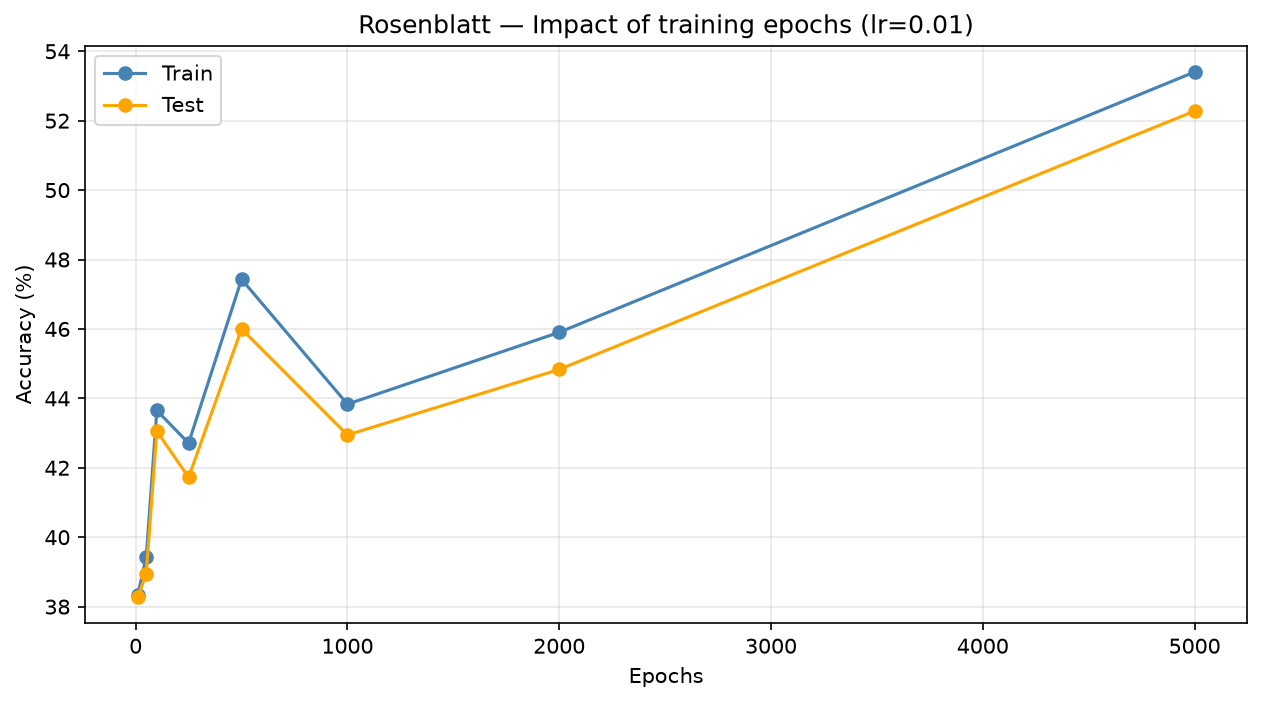
\includegraphics[width=0.85\linewidth]{report_plots/rosenblatt_epochs_sweep.png}
\caption{Rosenblatt --- Influence du nombre d'époques}
\end{figure}

\begin{center}\rule{0.5\linewidth}{0.5pt}\end{center}

\hypertarget{expuxe9rience-3-stabilituxe9-selon-la-graine-aluxe9atoire}{%
\section{Expérience 3 --- Stabilité selon la graine
aléatoire}\label{expuxe9rience-3-stabilituxe9-selon-la-graine-aluxe9atoire}}

Nous avons entraîné le modèle avec huit graines aléatoires différentes
en gardant les mêmes hyperparamètres, un taux d'apprentissage de 0,01 et
cinq cents époques. La précision de test moyenne s'établit à
quarante-deux virgule six pour cent, avec des variations allant
d'environ trente-neuf virgule sept pour cent pour la graine un jusqu'à
quarante-six pour cent pour la graine quarante-deux. L'écart entre la
meilleure et la pire graine atteint donc environ six points et trois
dixièmes.

Cette variabilité reste significative pour un modèle aussi simple et
s'explique par le fait que l'initialisation aléatoire des poids
détermine le point de départ dans l'espace des solutions. Comme le
perceptron ne dispose que de frontières linéaires, un mauvais point de
départ peut le conduire vers un hyperplan sous-optimal dont il ne pourra
jamais s'extraire, l'algorithme d'apprentissage ne garantissant la
convergence que lorsque les données sont linéairement séparables, ce qui
n'est pas le cas ici. Ce résultat suggère qu'en pratique, il serait
judicieux d'entraîner plusieurs modèles avec des graines différentes et
de conserver le meilleur.

\begin{figure}[htbp]
\centering
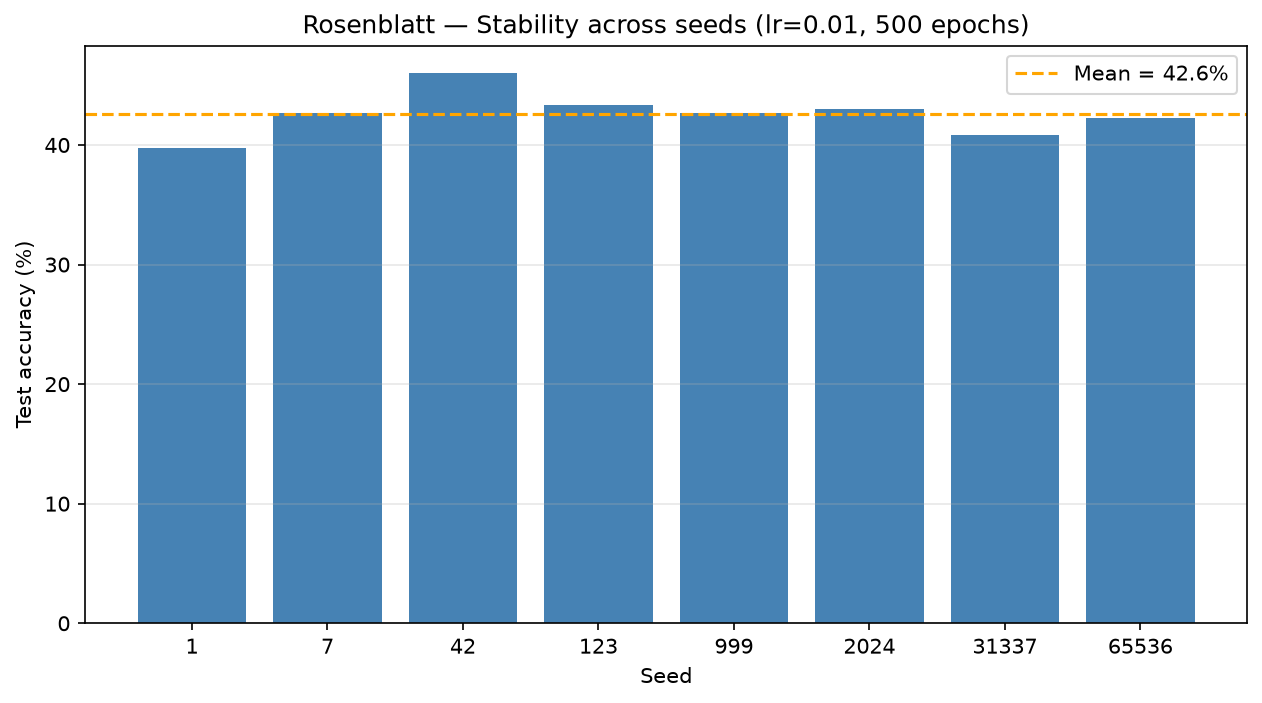
\includegraphics[width=0.85\linewidth]{report_plots/rosenblatt_seed_variance.png}
\caption{Rosenblatt --- Stabilité selon la graine aléatoire}
\end{figure}

\begin{center}\rule{0.5\linewidth}{0.5pt}\end{center}

\hypertarget{expuxe9rience-4-matrice-de-confusion}{%
\section{Expérience 4 --- Matrice de
confusion}\label{expuxe9rience-4-matrice-de-confusion}}

La matrice de confusion, obtenue avec un taux d'apprentissage de 0,01 et
cinq cents époques, révèle un problème majeur, différent de celui
observé lors d'une exécution précédente mais de même nature. Le modèle
prédit désormais la classe guépard dans la grande majorité des cas,
quelle que soit la vraie classe de l'image. Le guépard est correctement
reconnu dans environ quatre-vingt-quatorze pour cent des cas, avec cinq
cent soixante-quatre bonnes classifications sur cinq cent
quatre-vingt-dix-huit. Mais ce chiffre élevé est trompeur, car le lion
n'est correctement classé que dans environ sept pour cent des cas, avec
seulement quarante-deux bonnes classifications contre cinq cent
quarante-sept confusions avec le guépard. Le chat se situe entre les
deux, avec deux cent vingt-deux bonnes classifications sur cinq cent
quatre-vingt-neuf, soit environ trente-huit pour cent, la majorité de
ses erreurs étant elles aussi absorbées par le guépard plutôt que par le
lion.

Ce phénomène est celui d'un classifieur qui a convergé vers une solution
dégénérée, exactement comme lors de notre première observation, mais
avec un rôle différent attribué à chaque perceptron. Le perceptron
guépard a appris à répondre systématiquement oui, tandis que le
perceptron lion répond presque systématiquement non. Cette solution,
bien qu'elle paraisse absurde, est localement rationnelle pour un
classifieur linéaire : si la classe guépard représente un tiers des
exemples, prédire toujours guépard garantit mécaniquement environ
trente-trois pour cent de bonnes réponses sans avoir besoin de
distinguer quoi que ce soit. Le fait que la précision globale atteigne
quarante-six pour cent, nettement au-dessus de ce seuil, indique que le
perceptron chat parvient à intercepter une fraction substantielle des
chats, mais pas suffisamment pour produire un classifieur équilibré.

Ce résultat constitue à nouveau la démonstration la plus directe des
limites du perceptron simple sur notre problème, et le fait que la
classe qui absorbe les autres change d'une exécution à l'autre, lion
dans un cas, guépard dans l'autre, renforce plutôt qu'il n'affaiblit
cette conclusion : les trois classes de félins ne sont manifestement pas
séparables par des hyperplans dans l'espace des vingt caractéristiques
extraites, et le modèle retombe systématiquement vers une solution
dégénérée, sans qu'il soit possible de prédire à l'avance laquelle des
trois classes finira par absorber les deux autres. Cette instabilité de
la classe dominante fait elle-même écho à la sensibilité à la graine
aléatoire observée dans l'expérience précédente. Cette observation
contraste avec le MLP, dont la répartition des erreurs reste beaucoup
plus stable d'une exécution à l'autre, confirmant que la non-linéarité
des couches cachées est indispensable pour traiter ce problème de
manière satisfaisante et reproductible.

\begin{figure}[htbp]
\centering
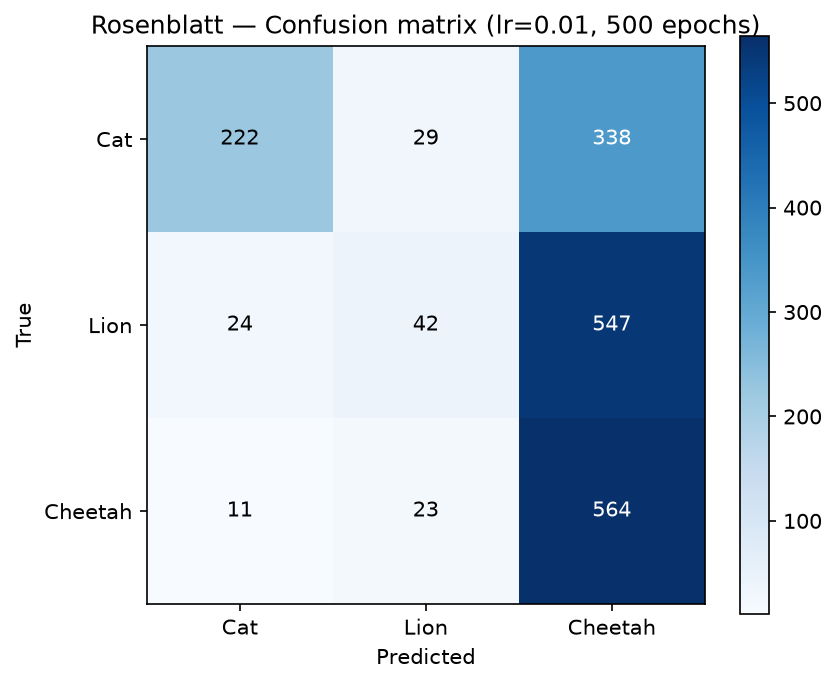
\includegraphics[width=0.85\linewidth]{report_plots/rosenblatt_confusion.png}
\caption{Rosenblatt --- Matrice de confusion}
\end{figure}

\begin{center}\rule{0.5\linewidth}{0.5pt}\end{center}

\hypertarget{synthuxe8se}{%
\section{Synthèse}\label{synthuxe8se}}

L'étude du perceptron de Rosenblatt met en lumière les limites
fondamentales d'un classifieur purement linéaire sur un problème de
classification visuelle. Le taux d'apprentissage optimal se dégage
nettement à 0,01, entouré d'un creux d'instabilité immédiatement après ;
l'entraînement prolongé jusqu'à cinq mille époques continue d'améliorer
les résultats sans signe de sur-apprentissage, signe qu'un classifieur
aussi peu paramétré ne mémorise pas ses exemples ; la sensibilité à
l'initialisation reste notable, avec un écart de plus de six points
entre graines ; et surtout, la matrice de confusion s'effondre
systématiquement vers une solution dégénérée qui ne distingue plus
vraiment les classes, la classe qui absorbe les deux autres changeant
d'une exécution à l'autre. Ces observations convergent vers la même
conclusion : le modèle manque de capacité expressive pour séparer trois
classes visuellement proches, et cette incapacité se traduit moins par
une précision uniformément basse que par une instabilité qualitative de
la solution trouvée. Avec une précision de test moyenne d'environ
quarante-deux à quarante-six pour cent selon la configuration, le
perceptron se situe nettement en deçà du MLP et des modèles non
linéaires, ce qui est cohérent avec la hiérarchie de complexité entre
ces modèles. Ce résultat justifie pleinement le recours à des
architectures non linéaires dans la suite du projet, tout en donnant au
perceptron le rôle de référence minimale auquel les modèles plus
élaborés doivent se comparer.

\begin{center}\rule{0.5\linewidth}{0.5pt}\end{center}

\hypertarget{uxe9tude-expuxe9rimentale-du-perceptron-multi-couches}{%
\chapter{Étude expérimentale du Perceptron
Multi-Couches}\label{uxe9tude-expuxe9rimentale-du-perceptron-multi-couches}}

\hypertarget{duxe9marche-de-construction-et-premiers-enseignements}{%
\section{Démarche de construction et premiers
enseignements}\label{duxe9marche-de-construction-et-premiers-enseignements}}

Avant de présenter les expériences systématiques, il faut retracer le
chemin qui a mené au modèle final, car il illustre à lui seul le
compromis biais-variance sur données réelles.

Le MLP est réparti en quatre fichiers : la structure principale avec les
méthodes forward, backward, train, predict et accuracy ; une couche
Dense avec ses poids, ses biais et sa fonction d'activation ; les
fonctions d'activation et leurs dérivées, tangente hyperbolique et ReLU
; et l'initialisation de He pour les poids. Les formules viennent
directement du cours : le delta de la couche de sortie vaut la dérivée
d'activation multipliée par l'écart entre sortie et cible, le delta des
couches cachées propage la somme pondérée des deltas suivants, et chaque
poids est mis à jour en retranchant le produit du taux d'apprentissage,
de l'entrée et du delta. Les cibles sont codées plus un pour la bonne
classe et moins un pour les autres, en cohérence avec la plage de sortie
de la tangente hyperbolique. Deux choix de conception méritent mention :
la fonction d'activation est portée par chaque couche sous forme de
pointeur de fonction, et l'activation de sortie est un paramètre
distinct de celle des couches cachées, si bien que le même code sert à
la classification comme à la régression ; l'architecture elle-même est
un simple tableau de tailles de couches passé au constructeur.

La première campagne d'entraînement sur images réelles, menée en pixels
bruts sur six cents images seulement avec une architecture à trois mille
soixante-douze entrées, a produit soixante-quinze pour cent en
apprentissage contre quarante-deux et demi pour cent en test : un
sur-apprentissage massif, parfaitement prévisible avec environ
quarante-neuf mille paramètres pour quatre cent quatre-vingts exemples
d'apprentissage, soit plus de cent fois en dessous de la règle du cours
qui recommande dix fois plus d'exemples que de paramètres.
L'augmentation du jeu à neuf mille images a fait disparaître l'écart,
quarante-huit pour cent des deux côtés, mais en basculant dans l'excès
inverse : un modèle sous-ajusté, à peine au-dessus du hasard, ses
dizaines de milliers de paramètres n'apprenant rien d'utile en un temps
raisonnable. C'est ce double échec qui a motivé les vingt
caractéristiques extraites : avec une architecture à vingt entrées,
seize neurones cachés et trois sorties, soit environ quatre cents
paramètres pour sept mille deux cents exemples, le budget de paramètres
est largement respecté et le modèle atteint cinquante-huit pour cent en
apprentissage pour cinquante-six en test, un écart inférieur à deux
points qui est le profil d'un modèle sain. Un essai avec une
architecture plus profonde a fait grimper l'apprentissage de trois
points sans bouger le test, confirmant que la capacité supplémentaire
partait en sur-apprentissage.

\hypertarget{expuxe9riences-systuxe9matiques}{%
\section{Expériences
systématiques}\label{expuxe9riences-systuxe9matiques}}

\hypertarget{cadre-muxe9thodologique-1}{%
\section{Cadre méthodologique}\label{cadre-muxe9thodologique-1}}

Dans cette partie, nous étudions le comportement de notre implémentation
du Perceptron Multi-Couches sur le jeu de données felidae, qui regroupe
des images de chats, de lions et de guépards. Chaque image est d'abord
réduite à une taille de 32×32 pixels puis transformée en un vecteur de
vingt caractéristiques par notre fonction d'extraction. Ces vingt
caractéristiques regroupent la moyenne et l'écart-type de chaque canal
de couleur, un histogramme de luminosité à huit intervalles, et une
mesure de densité de contours à deux seuils. Ce choix de représentation
compacte, plutôt qu'un aplatissement brut des pixels, respecte la
contrainte que nous nous sommes fixée de ne jamais dépasser un nombre de
caractéristiques supérieur à dix pour cent de la taille du jeu
d'apprentissage.

Toutes les expériences qui suivent isolent un seul paramètre à la fois,
de manière à mettre en évidence son influence propre sur la vitesse de
convergence et sur la capacité de généralisation du modèle. Sauf mention
contraire, nous utilisons une architecture de référence à deux couches
cachées de trente-deux et seize neurones, un taux d'apprentissage de
0,01, et une fonction d'activation tangente hyperbolique. Le découpage
entre apprentissage et test suit une répartition de quatre-vingts pour
cent contre vingt pour cent. Chaque configuration a été journalisée dans
TensorBoard afin de conserver la trace de la perte, de la précision
d'apprentissage et de la précision de test à chaque époque.

\hypertarget{expuxe9rience-1-influence-du-taux-dapprentissage-1}{%
\section{Expérience 1 --- Influence du taux
d'apprentissage}\label{expuxe9rience-1-influence-du-taux-dapprentissage-1}}

Nous avons d'abord fait varier le taux d'apprentissage sur six valeurs
allant de 0,001 à 0,5, en gardant l'architecture et le nombre d'époques
fixes à deux cents. Les résultats montrent une plage optimale étroite.
Les meilleures précisions de test se situent autour de 0,005 et 0,01,
avec environ soixante-cinq pour cent, tandis que les valeurs plus
faibles convergent trop lentement pour atteindre leur plein potentiel en
deux cents époques seulement.

Le phénomène le plus parlant apparaît du côté des taux élevés. À 0,1, la
précision chute déjà à environ cinquante et un pour cent, et à 0,5 le
réseau tombe à trente et un pour cent, c'est-à-dire en dessous du seuil
aléatoire de trente-trois pour cent qu'obtiendrait un classifieur qui
répondrait au hasard entre trois classes. Cette dégradation illustre
l'instabilité des pas de gradient trop grands : les mises à jour de
poids deviennent si importantes qu'elles font diverger l'apprentissage
au lieu de le faire converger. Cette expérience justifie à elle seule
pourquoi nous retenons un taux d'apprentissage modéré dans la suite du
projet.

\begin{figure}[htbp]
\centering
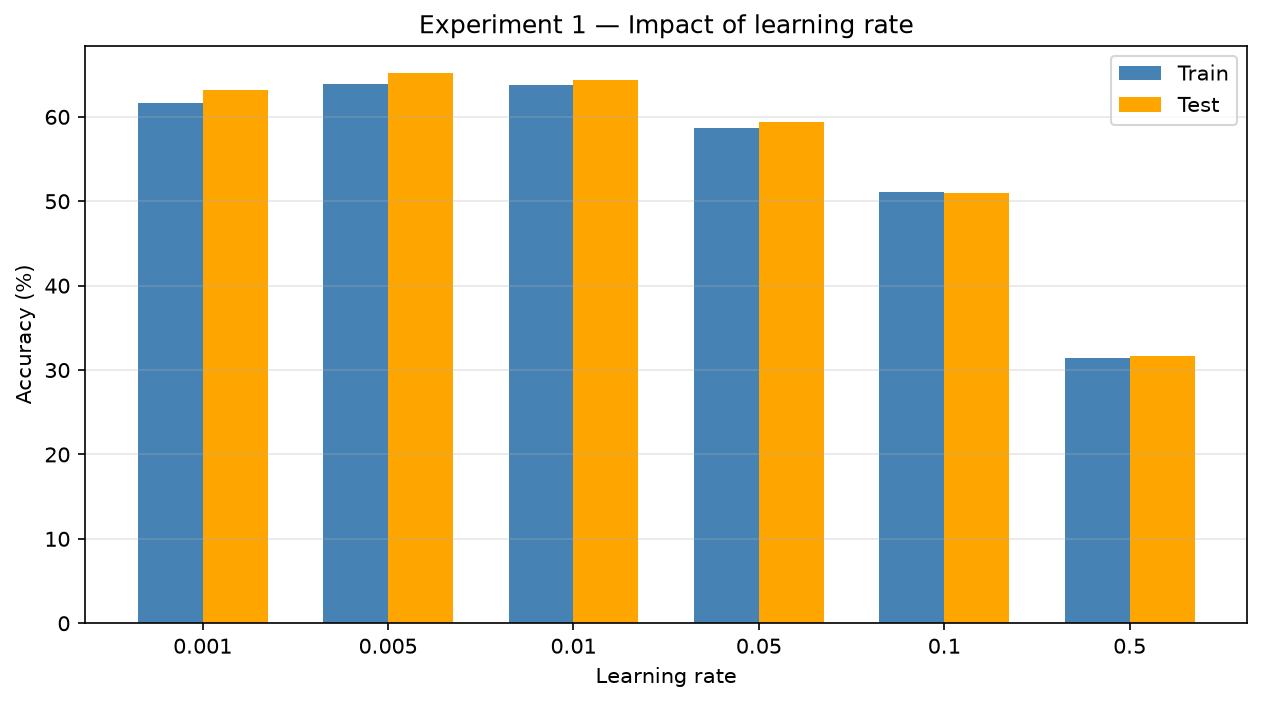
\includegraphics[width=0.85\linewidth]{report_plots/exp1_learning_rate.png}
\caption{Expérience 1 --- Influence du taux d'apprentissage}
\end{figure}

\hypertarget{expuxe9rience-2-influence-du-nombre-duxe9poques-1}{%
\section{Expérience 2 --- Influence du nombre
d'époques}\label{expuxe9rience-2-influence-du-nombre-duxe9poques-1}}

Nous avons ensuite observé l'évolution des deux précisions en fonction
du nombre d'époques, de dix jusqu'à deux mille. La courbe reproduit le
comportement classique décrit en cours. Dans les premières époques, les
deux précisions montent ensemble : le modèle est en situation de
sous-apprentissage et progresse encore. La précision de test atteint son
maximum, environ soixante-cinq et demi pour cent, autour de deux cent
cinquante époques.

Au-delà de ce point, les deux courbes divergent. La précision
d'apprentissage continue de croître régulièrement jusqu'à près de
soixante-neuf pour cent, alors que la précision de test redescend et
devient irrégulière. Cette divergence est la signature même du
sur-apprentissage : le réseau se met à mémoriser les particularités du
jeu d'apprentissage au lieu d'apprendre des régularités transférables.
Le point situé autour de deux cent cinquante époques représente donc le
compromis que le sujet nous demande d'identifier, celui d'un modèle
suffisamment complexe pour bien traiter les données d'apprentissage mais
encore assez simple pour généraliser correctement.

\begin{figure}[htbp]
\centering
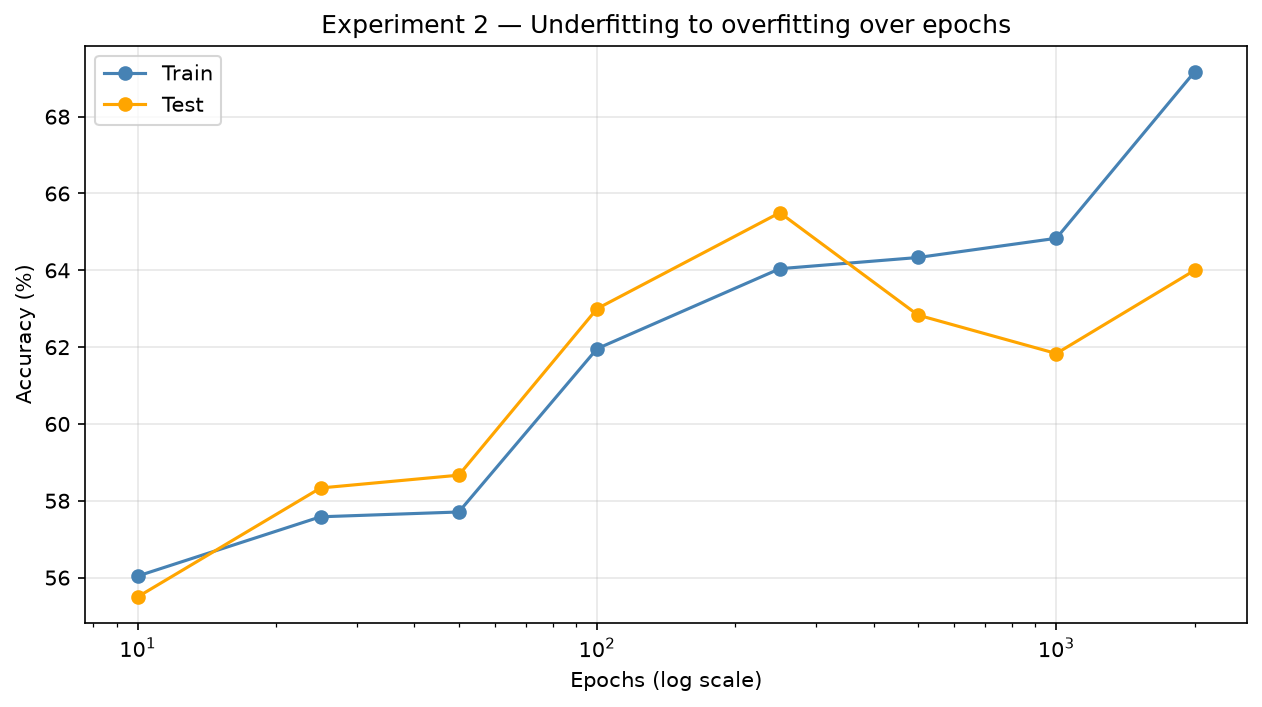
\includegraphics[width=0.85\linewidth]{report_plots/exp2_epochs.png}
\caption{Expérience 2 --- Du sous-apprentissage au sur-apprentissage
selon le nombre d'époques}
\end{figure}

\hypertarget{expuxe9rience-3-influence-de-la-profondeur-du-ruxe9seau}{%
\section{Expérience 3 --- Influence de la profondeur du
réseau}\label{expuxe9rience-3-influence-de-la-profondeur-du-ruxe9seau}}

Pour mesurer l'effet de la profondeur, nous avons comparé six
architectures, depuis un réseau sans couche cachée jusqu'à un réseau à
trois couches cachées de cent vingt-huit, soixante-quatre et trente-deux
neurones. Le résultat est instructif par sa sobriété : la profondeur
n'apporte qu'un gain marginal. Le passage d'un modèle purement linéaire,
à environ soixante-deux et demi pour cent de précision de test, à
l'architecture la plus profonde, à environ soixante-cinq pour cent, ne
représente qu'une amélioration de deux points et demi.

Nous en tirons une conclusion importante pour l'analyse critique du
projet. Le facteur limitant n'est pas la capacité du réseau mais la
richesse des vingt caractéristiques extraites. Une fois que le modèle a
exploité l'information contenue dans ces caractéristiques, ajouter des
couches ne lui donne pas matière à mieux séparer les classes. Cette
observation oriente naturellement les pistes d'amélioration vers une
représentation d'entrée plus riche plutôt que vers un réseau plus
profond.

\begin{figure}[htbp]
\centering
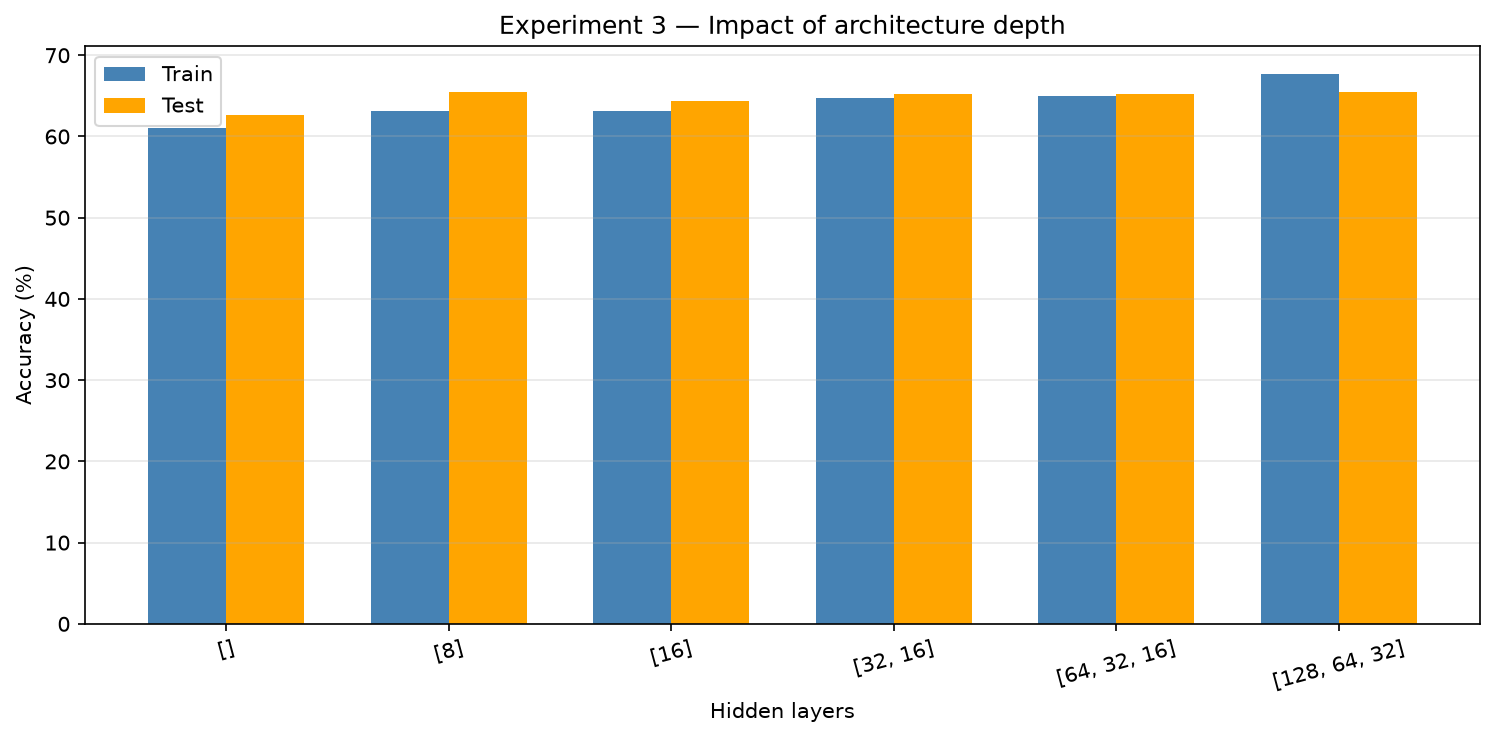
\includegraphics[width=0.85\linewidth]{report_plots/exp3_depth.png}
\caption{Expérience 3 --- Influence de la profondeur du réseau}
\end{figure}

\hypertarget{expuxe9rience-4-influence-de-la-taille-du-jeu-de-donnuxe9es}{%
\section{Expérience 4 --- Influence de la taille du jeu de
données}\label{expuxe9rience-4-influence-de-la-taille-du-jeu-de-donnuxe9es}}

Cette expérience est celle qui met le plus clairement en évidence le
lien entre quantité de données et généralisation. Nous avons fait varier
le nombre d'exemples par classe de cinquante jusqu'à trois mille, en
conservant un ensemble de test fixe. Avec seulement cinquante exemples
par classe, l'écart entre précision d'apprentissage et précision de test
atteint quinze virgule six points : le modèle apprend presque
parfaitement ses quelques exemples mais généralise mal, ce qui est la
définition même du sur-apprentissage sur données rares.

À mesure que nous augmentons la taille du jeu, cet écart se réduit
fortement. Il devient minimal, environ un point, autour de mille
exemples par classe, taille qui offre également la meilleure précision
de test avec environ soixante et un et demi pour cent. Au-delà, les
gains se stabilisent. Cette expérience fournit la justification
empirique de la taille de jeu que nous avons retenue pour l'entraînement
final : c'est le point où le modèle cesse de sur-apprendre sans qu'un
ajout de données ne change plus grand-chose.

\begin{figure}[htbp]
\centering
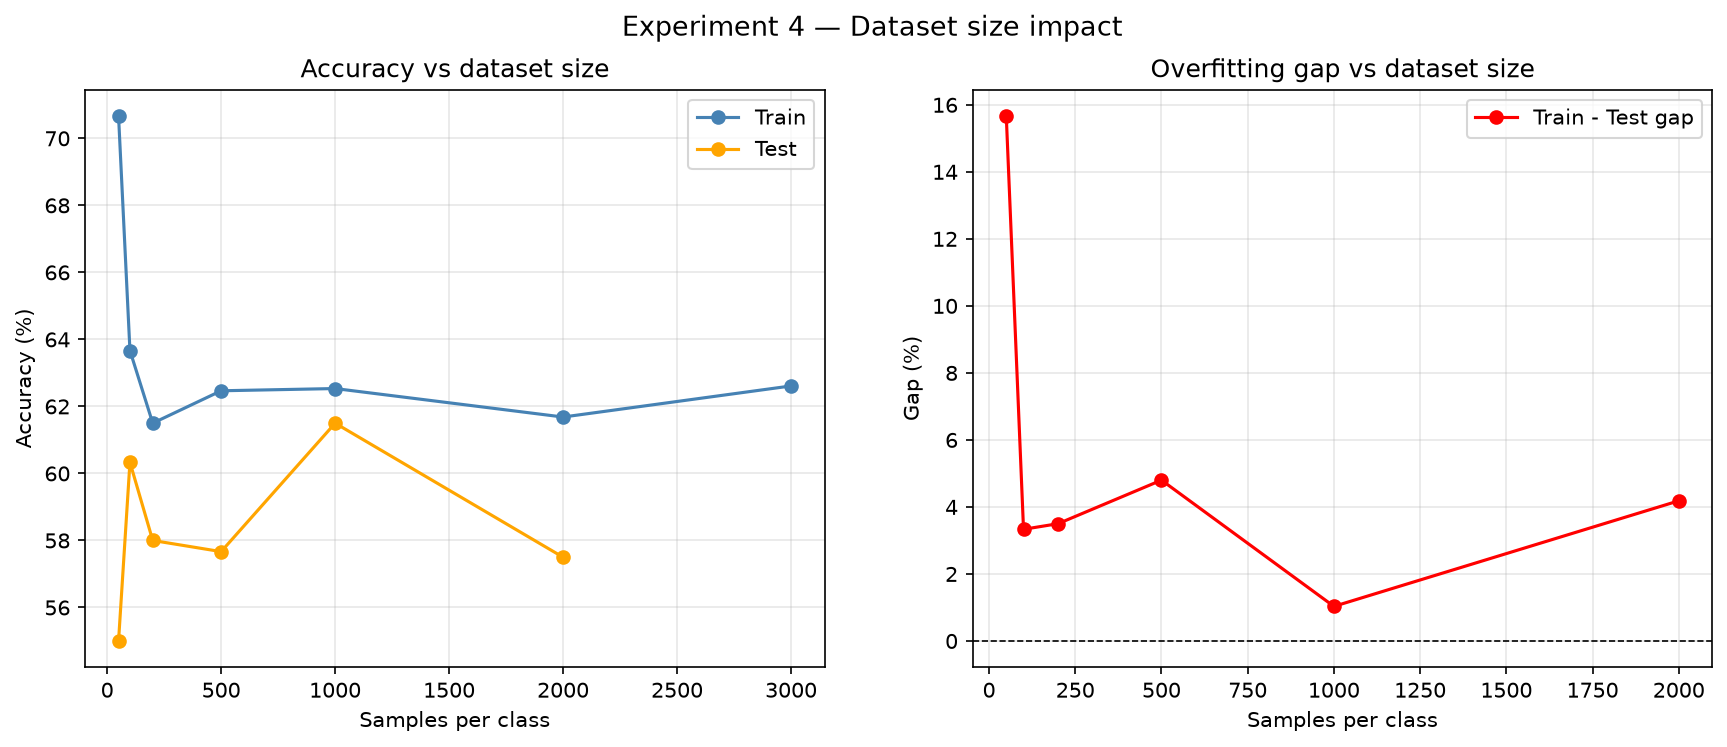
\includegraphics[width=0.85\linewidth]{report_plots/exp4_dataset_size.png}
\caption{Expérience 4 --- Influence de la taille du jeu de données}
\end{figure}

\hypertarget{expuxe9rience-5-mise-en-uxe9vidence-du-sur-apprentissage}{%
\section{Expérience 5 --- Mise en évidence du
sur-apprentissage}\label{expuxe9rience-5-mise-en-uxe9vidence-du-sur-apprentissage}}

Pour isoler le sur-apprentissage de manière volontairement caricaturale,
nous avons entraîné un réseau volumineux, à trois couches cachées de
cent vingt-huit, soixante-quatre et trente-deux neurones, sur un jeu
délibérément minuscule de cinquante exemples par classe. Le résultat est
sans ambiguïté. La précision d'apprentissage grimpe jusqu'à cent pour
cent au fil des époques, ce qui signifie que le réseau finit par
mémoriser parfaitement chaque exemple. Pendant ce temps, la précision de
test reste bloquée autour de quarante à quarante-cinq pour cent.

La zone colorée entre les deux courbes, qui s'élargit continûment,
matérialise visuellement le sur-apprentissage. C'est l'illustration la
plus directe du principe selon lequel un modèle trop puissant pour la
quantité de données disponible apprend le bruit plutôt que le signal.
Cette figure est particulièrement utile en soutenance car elle rend le
phénomène immédiatement lisible.

\begin{figure}[htbp]
\centering
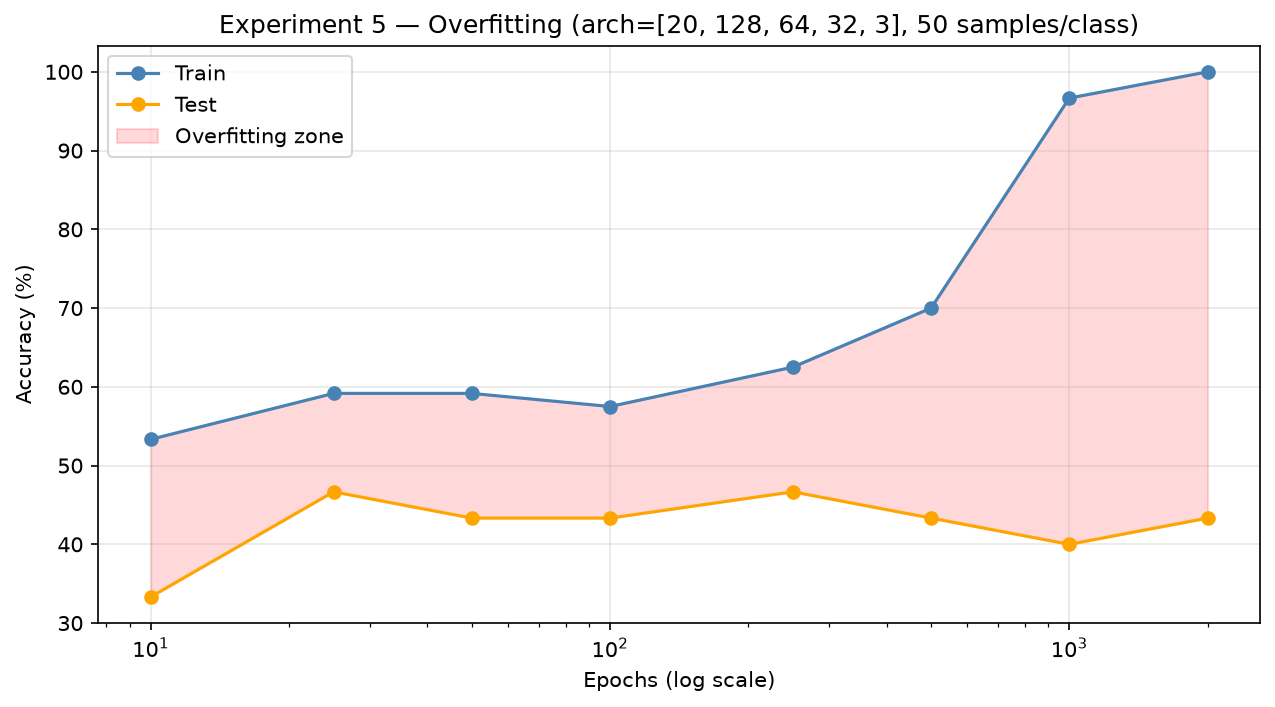
\includegraphics[width=0.85\linewidth]{report_plots/exp5_overfitting.png}
\caption{Expérience 5 --- Mise en évidence du sur-apprentissage}
\end{figure}

\hypertarget{expuxe9rience-6-mise-en-uxe9vidence-du-sous-apprentissage}{%
\section{Expérience 6 --- Mise en évidence du
sous-apprentissage}\label{expuxe9rience-6-mise-en-uxe9vidence-du-sous-apprentissage}}

À l'inverse, nous avons cherché à provoquer le sous-apprentissage en
réduisant le réseau à une unique couche cachée de deux neurones
seulement. Nous devons toutefois nuancer le résultat par honnêteté
intellectuelle. Même avec ce goulot d'étranglement extrême, le réseau
atteint environ soixante-deux pour cent de précision de test, très
au-dessus du seuil aléatoire de trente-trois pour cent.

Ce sous-apprentissage est donc réel mais modéré, et il s'explique par la
même raison que l'expérience sur la profondeur : les vingt
caractéristiques que nous extrayons sont déjà si informatives qu'un
réseau minimal parvient encore à en tirer beaucoup. Autrement dit, la
difficulté du problème réside davantage dans la qualité de la
représentation que dans la capacité du classifieur. Ce constat renforce
l'analyse que nous portons sur l'ensemble du projet.

\begin{figure}[htbp]
\centering
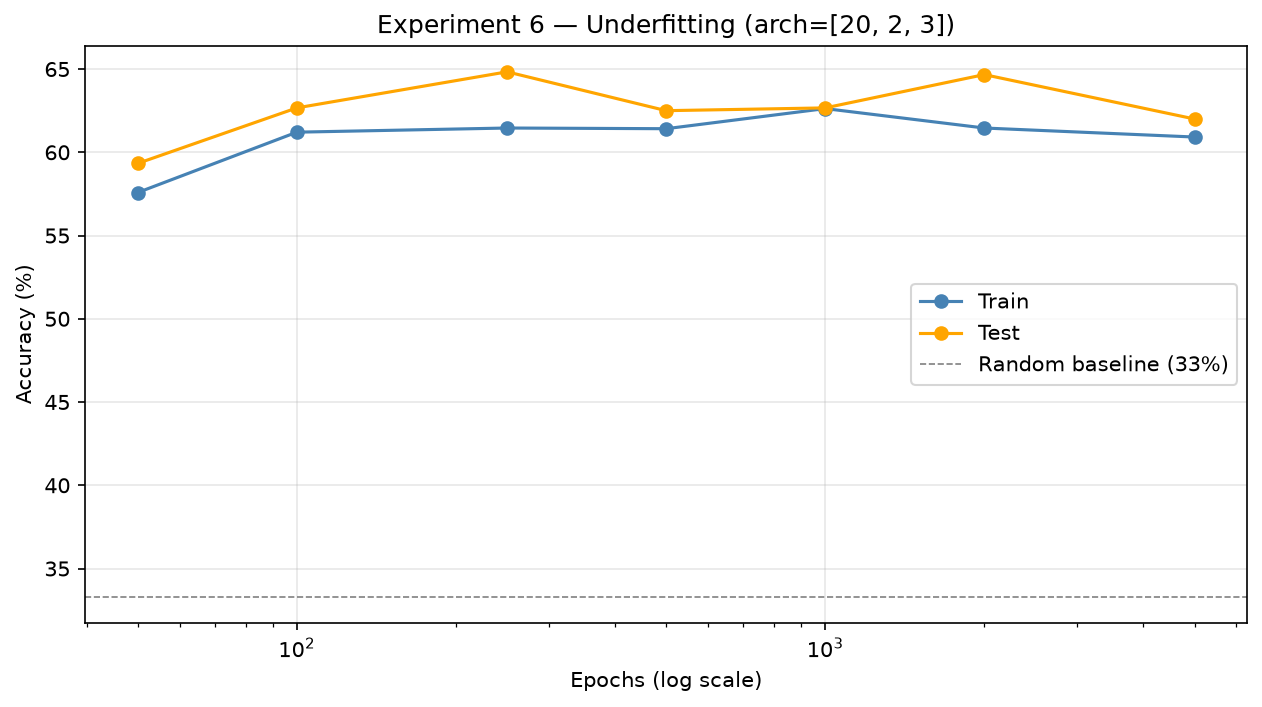
\includegraphics[width=0.85\linewidth]{report_plots/exp6_underfitting.png}
\caption{Expérience 6 --- Mise en évidence du sous-apprentissage}
\end{figure}

\hypertarget{expuxe9rience-7-recherche-du-compromis-par-architecture}{%
\section{Expérience 7 --- Recherche du compromis par
architecture}\label{expuxe9rience-7-recherche-du-compromis-par-architecture}}

Cette dernière expérience synthétise les deux précédentes en croisant
profondeur et nombre d'époques. Pour quatre architectures de complexité
croissante, nous avons tracé l'évolution des deux précisions en fonction
du nombre d'époques. Les quatre panneaux racontent une histoire
cohérente : quelle que soit l'architecture, la précision de test culmine
autour de deux cent cinquante époques puis décline.

Le point remarquable est que ce déclin est d'autant plus marqué que le
réseau est volumineux. Pour l'architecture la plus grande, à cent
vingt-huit, soixante-quatre et trente-deux neurones, la précision de
test chute d'environ soixante-cinq pour cent à soixante-deux pour cent
tandis que sa précision d'apprentissage grimpe jusqu'à soixante-dix pour
cent. Un réseau plus grand sur-apprend donc plus vite et plus fort, ce
qui confirme le lien entre capacité du modèle et vitesse d'apparition du
sur-apprentissage. Cette figure relie proprement les enseignements des
expériences deux et trois.

\begin{figure}[htbp]
\centering
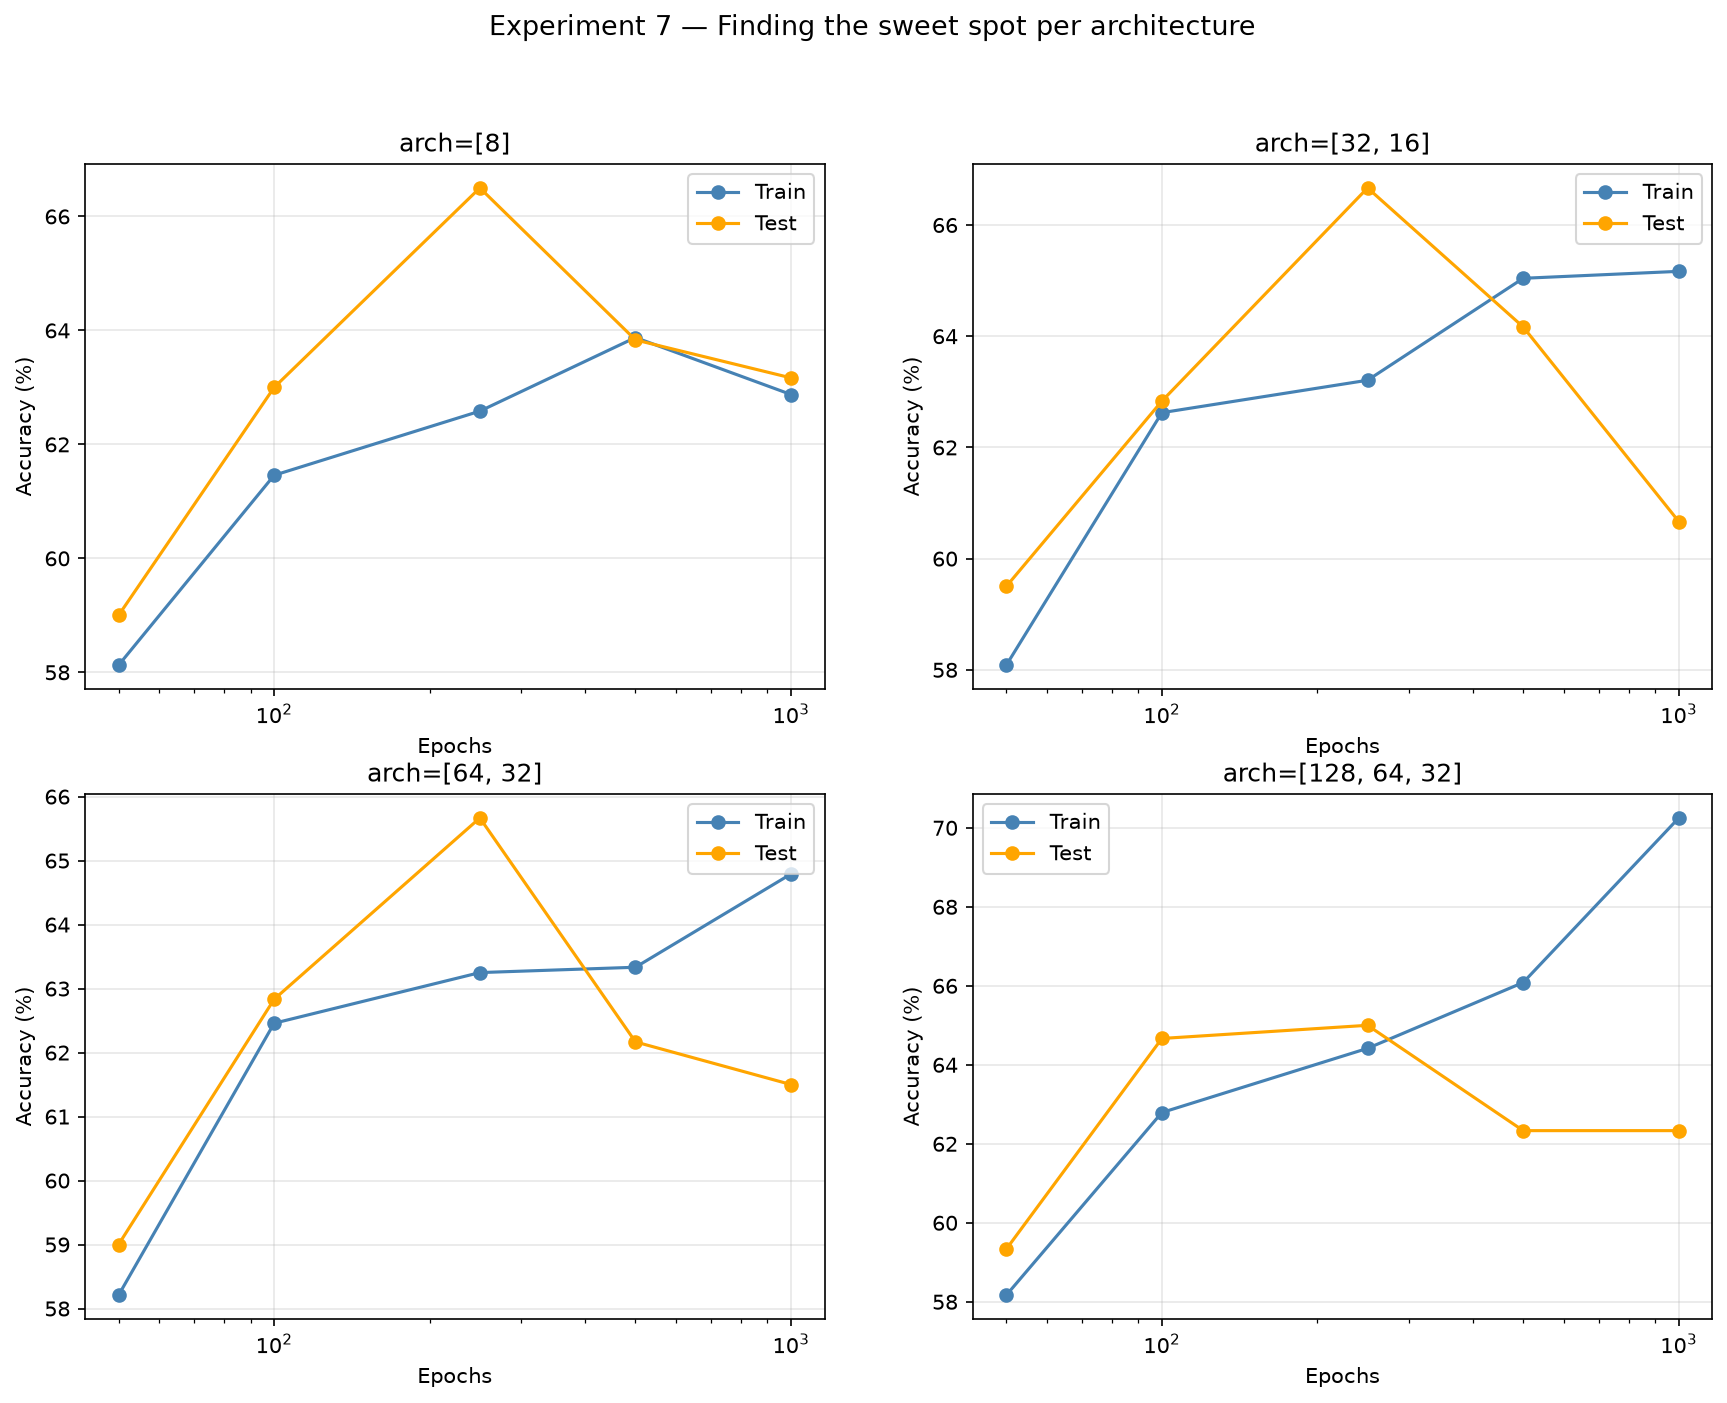
\includegraphics[width=0.85\linewidth]{report_plots/exp7_sweet_spot.png}
\caption{Expérience 7 --- Recherche du compromis par architecture}
\end{figure}

\hypertarget{expuxe9rience-8-matrice-de-confusion-du-meilleur-moduxe8le}{%
\section{Expérience 8 --- Matrice de confusion du meilleur
modèle}\label{expuxe9rience-8-matrice-de-confusion-du-meilleur-moduxe8le}}

Pour terminer, nous avons entraîné le modèle dans sa configuration de
référence et nous avons examiné la matrice de confusion sur l'ensemble
de test. La précision globale s'établit autour de soixante-quatre pour
cent, avec des performances très inégales selon les classes. Le chat est
reconnu correctement dans environ soixante-neuf pour cent des cas, et le
lion dans environ soixante et onze pour cent des cas. Le guépard est en
revanche la classe la plus difficile, avec seulement cinquante et un
pour cent de bonnes classifications.

La source principale d'erreur est identifiable sans ambiguïté :
soixante-dix-neuf guépards sont confondus avec des lions, contre cent
deux correctement classés. Cette confusion entre lion et guépard est
parfaitement compréhensible sur le plan visuel, puisque les deux animaux
partagent une fourrure fauve, une morphologie proche et souvent un décor
de savane similaire. Le chat, avec ses couleurs et ses contextes plus
variés, se distingue plus facilement. Cette analyse par classe est plus
riche qu'un simple chiffre global car elle indique précisément où le
modèle échoue et pourquoi, ce qui ouvre des pistes concrètes
d'amélioration comme l'ajout de caractéristiques de texture plus fines
capables de distinguer les motifs de pelage.

\begin{figure}[htbp]
\centering
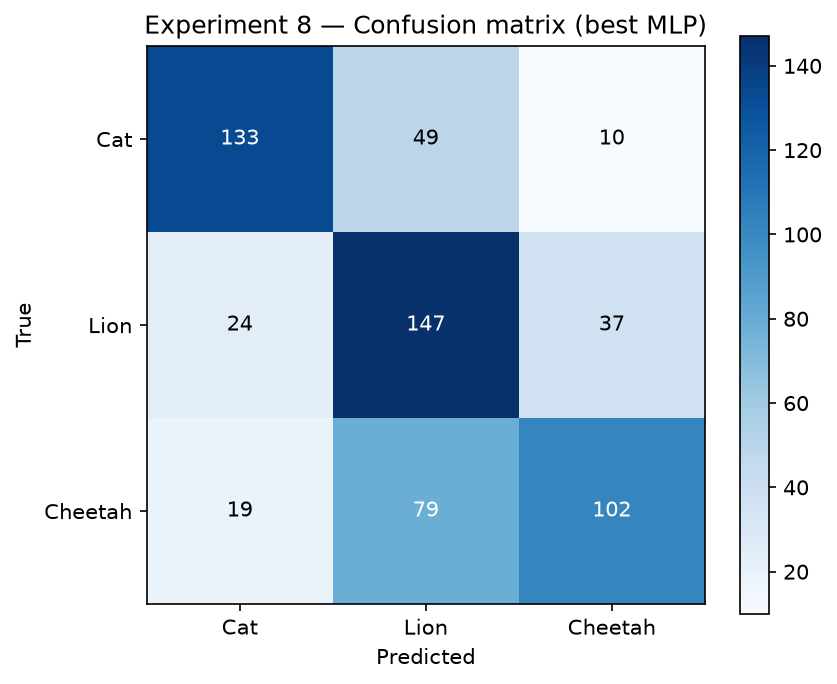
\includegraphics[width=0.85\linewidth]{report_plots/exp8_confusion.png}
\caption{Expérience 8 --- Matrice de confusion du meilleur modèle}
\end{figure}

\hypertarget{comparaison-des-repruxe9sentations-dentruxe9e-caractuxe9ristiques-extraites-contre-pixels-bruts}{%
\section{Comparaison des représentations d'entrée : caractéristiques
extraites contre pixels
bruts}\label{comparaison-des-repruxe9sentations-dentruxe9e-caractuxe9ristiques-extraites-contre-pixels-bruts}}

Jusqu'ici, toutes nos expériences reposaient sur les vingt
caractéristiques extraites. Nous avons voulu mesurer ce que le modèle
apprend lorsqu'on lui fournit à la place les pixels bruts de l'image,
c'est-à-dire une image redimensionnée en 32×32 en couleur, soit trois
mille soixante-douze valeurs par exemple. Nous entraînons dans les deux
cas la même architecture pendant cent époques au même taux
d'apprentissage, et nous comparons les résultats.

En pixels bruts, le modèle atteint soixante-trois virgule trois pour
cent en apprentissage et cinquante-quatre virgule deux pour cent en
test, contre environ soixante-quatre pour cent en apprentissage et
cinquante-deux pour cent en test pour les caractéristiques extraites.
Les pixels bruts généralisent donc légèrement mieux, ce qui s'explique
simplement : ils transportent davantage d'information brute que nos
vingt descripteurs globaux. Ce gain a toutefois un coût. Avec trois
mille soixante-douze caractéristiques pour sept mille deux cents
exemples d'apprentissage, cette configuration viole la contrainte que
nous nous étions fixée de ne pas dépasser dix pour cent de la taille du
jeu, et son entraînement est nettement plus lourd. La représentation par
caractéristiques extraites reste donc celle qui respecte la règle du
projet, les pixels bruts n'étant présentés qu'à titre de comparaison.

L'observation la plus intéressante ne porte pas sur la précision globale
mais sur la matrice de confusion. En pixels bruts, le chat devient la
classe la mieux reconnue, avec quatre cent quarante-trois exemples
correctement classés, tandis que le lion devient la classe la plus
faible, deux cent soixante lions étant confondus avec des chats. C'est
exactement l'inverse de ce que nous observons avec les caractéristiques
extraites, où le lion était bien séparé. Autrement dit, le choix de la
représentation d'entrée ne déplace pas seulement la précision de
quelques points : il change la classe sur laquelle le modèle échoue. Les
caractéristiques extraites séparent bien le lion, les pixels bruts
séparent bien le chat, et aucune des deux représentations n'est
uniformément supérieure à l'autre. Ce constat illustre concrètement que
la performance d'un modèle dépend autant de la manière dont on lui
présente les données que du modèle lui-même.

\hypertarget{synthuxe8se-1}{%
\section{Synthèse}\label{synthuxe8se-1}}

L'ensemble de ces expériences met en évidence, sur notre propre modèle
et notre propre jeu de données, les phénomènes fondamentaux étudiés en
cours. Nous observons une plage étroite de taux d'apprentissage viable
et une divergence brutale au-delà, un compromis temporel situé autour de
deux cent cinquante époques, un sur-apprentissage d'autant plus rapide
que le réseau est grand ou que les données sont rares, et un
sous-apprentissage réel mais atténué par la qualité de nos
caractéristiques. Le plafond de performance, autour de soixante-quatre
pour cent, s'explique moins par les limites du perceptron lui-même que
par la difficulté intrinsèque à distinguer trois félins à partir de
vingt caractéristiques globales. Cette conclusion est celle qui nous
semble la plus utile à défendre : la performance d'un système
d'apprentissage dépend au moins autant de la représentation des données
que du modèle qui les traite.

\begin{center}\rule{0.5\linewidth}{0.5pt}\end{center}

\hypertarget{uxe9tude-expuxe9rimentale-du-radial-basis-function-network}{%
\chapter{Étude expérimentale du Radial Basis Function
Network}\label{uxe9tude-expuxe9rimentale-du-radial-basis-function-network}}

\hypertarget{cadre-muxe9thodologique-2}{%
\section{Cadre méthodologique}\label{cadre-muxe9thodologique-2}}

Le Radial Basis Function Network repose sur une idée différente de celle
du perceptron. Plutôt que d'ajuster progressivement des poids par
descente de gradient, il conserve un ensemble de points de référence et
attribue à chacun une zone d'influence en forme de cloche gaussienne.
L'influence ressentie en un point \(X\) par un centre \(\mu\) vaut
\(e^{-\gamma \|X - \mu\|^2}\) : elle vaut un exactement sur le centre et
décroît vers zéro à mesure que l'on s'en éloigne. La sortie du réseau
est la somme pondérée de toutes ces cloches, et pour la classification
nous prenons la classe dont la somme est la plus forte.

Le paramètre gamma contrôle la largeur des cloches. Un gamma élevé
produit des pics étroits, où chaque centre n'influence que son voisinage
immédiat, tandis qu'un gamma faible produit des dômes larges qui
s'étalent sur tout l'espace. Ce paramètre joue donc pour le RBFN le même
rôle d'arbitrage entre sur-apprentissage et sous-apprentissage que le
nombre d'époques jouait pour le perceptron.

Nous n'utilisons pas la version naïve, qui conserverait chaque exemple
comme centre et produirait autant de poids que d'exemples, ce que le
cours signale comme un mauvais présage pour la généralisation. Nous
élisons à la place un nombre réduit de \(K\) centres représentatifs à
l'aide de l'algorithme de Lloyd, une méthode de k-means qui répète deux
étapes jusqu'à stabilisation : assigner chaque exemple à son centre le
plus proche, puis déplacer chaque centre vers la moyenne des exemples
qui lui sont assignés. Les poids sont ensuite obtenus en une seule
opération par la pseudo-inverse \(W = (\Phi^T\Phi)^{-1}\Phi^T Y\), où la
matrice \(\Phi\) contient l'influence de chaque centre sur chaque
exemple. L'entraînement du RBFN n'a donc pas de boucle d'époques : il
consiste à trouver les centres puis à résoudre un seul système linéaire.

En haute dimension, la matrice \(\Phi^T\Phi\) peut devenir singulière,
c'est-à-dire non inversible, car de nombreuses colonnes de \(\Phi\)
prennent des valeurs presque identiques. Pour garantir l'inversibilité,
nous ajoutons un terme de régularisation en ajoutant une petite valeur
sur la diagonale avant l'inversion, ce qui revient à résoudre
\(W = (\Phi^T\Phi + \lambda I)^{-1}\Phi^T Y\). Ce terme minuscule suffit
à stabiliser le calcul sans altérer sensiblement la solution.

Les résultats présentés ici utilisent la représentation par pixels
bruts, car c'est dans cet espace de grande dimension que les phénomènes
décrits en cours apparaissent le plus clairement. La représentation par
caractéristiques extraites donne des courbes plus plates, que nous
mentionnons en comparaison.

\hypertarget{expuxe9rience-1-influence-de-gamma}{%
\section{Expérience 1 --- Influence de
gamma}\label{expuxe9rience-1-influence-de-gamma}}

Nous avons fait varier gamma sur huit valeurs, de 0,001 à 10, en gardant
cinquante centres. La courbe suit cette fois le comportement théorique
attendu. La précision atteint son maximum autour de gamma égal à 0,01,
avec environ cinquante-six pour cent en apprentissage et
cinquante-quatre pour cent en test. Pour les valeurs plus faibles, les
cloches sont trop larges et se recouvrent au point que tous les centres
se ressemblent, ce qui empêche le réseau de distinguer les régions :
c'est du sous-apprentissage. Pour les valeurs plus élevées, la précision
décline puis s'effondre jusqu'au seuil aléatoire de trente-trois pour
cent à gamma égal à 5 et 10.

Cet effondrement est la signature de la mémorisation extrême : avec des
cloches devenues des pics infiniment fins, chaque centre n'a plus
d'influence que sur lui-même, si bien qu'un point de test qui ne tombe
pas exactement sur un centre ne reçoit aucune influence et ne peut être
classé. Il est notable que ce régime d'effondrement n'apparaît que dans
l'espace de grande dimension des pixels bruts. Avec les caractéristiques
extraites, en dimension vingt, la précision se contentait de monter puis
de se stabiliser sans jamais s'effondrer, car les centres y restent
toujours assez proches pour que leurs cloches se recouvrent. La
dimension de l'espace détermine donc si le régime de sur-apprentissage
est seulement atteignable.

\begin{figure}[htbp]
\centering
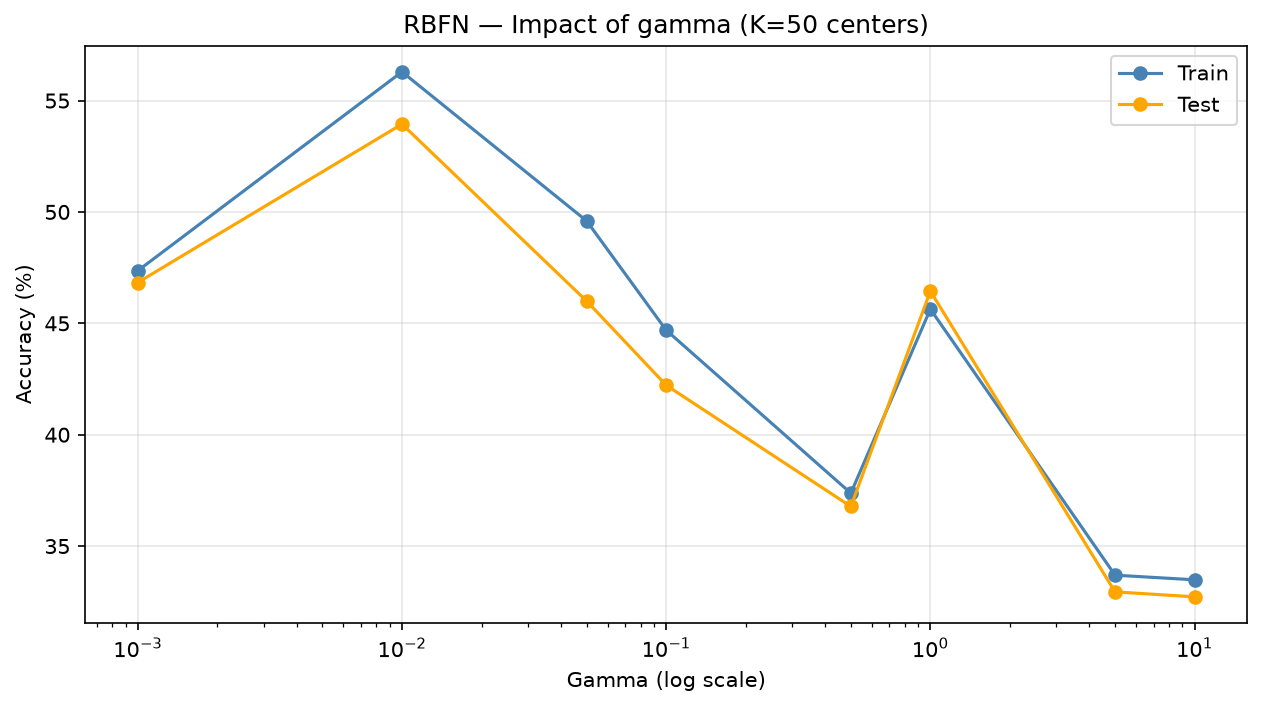
\includegraphics[width=0.85\linewidth]{report_plots/rbfn_gamma_sweep.png}
\caption{RBFN --- Influence de gamma}
\end{figure}

\hypertarget{expuxe9rience-2-influence-du-nombre-de-centres}{%
\section{Expérience 2 --- Influence du nombre de
centres}\label{expuxe9rience-2-influence-du-nombre-de-centres}}

Nous avons ensuite fait varier le nombre de centres \(K\) de deux à
quatre cents, à gamma fixé. Avec très peu de centres, le réseau reste au
niveau aléatoire, car deux ou cinq cloches ne suffisent pas à couvrir un
espace de trois mille dimensions. La précision monte régulièrement à
mesure que nous ajoutons des centres, atteignant environ cinquante pour
cent en test autour de deux cents centres. Ce besoin d'un grand nombre
de centres contraste avec la représentation par caractéristiques
extraites, où la précision culminait dès une dizaine de centres : en
basse dimension, peu de représentants suffisent à couvrir l'espace,
alors qu'en haute dimension il en faut beaucoup plus.

Le début d'un écart entre apprentissage et test apparaît aux valeurs
élevées de \(K\) : à quatre cents centres, l'apprentissage atteint près
de cinquante-cinq pour cent tandis que le test plafonne autour de
quarante-neuf pour cent. Cet écart naissant illustre le principe du
cours selon lequel augmenter le nombre de paramètres, ici le nombre de
centres, finit par nuire à la généralisation.

\begin{figure}[htbp]
\centering
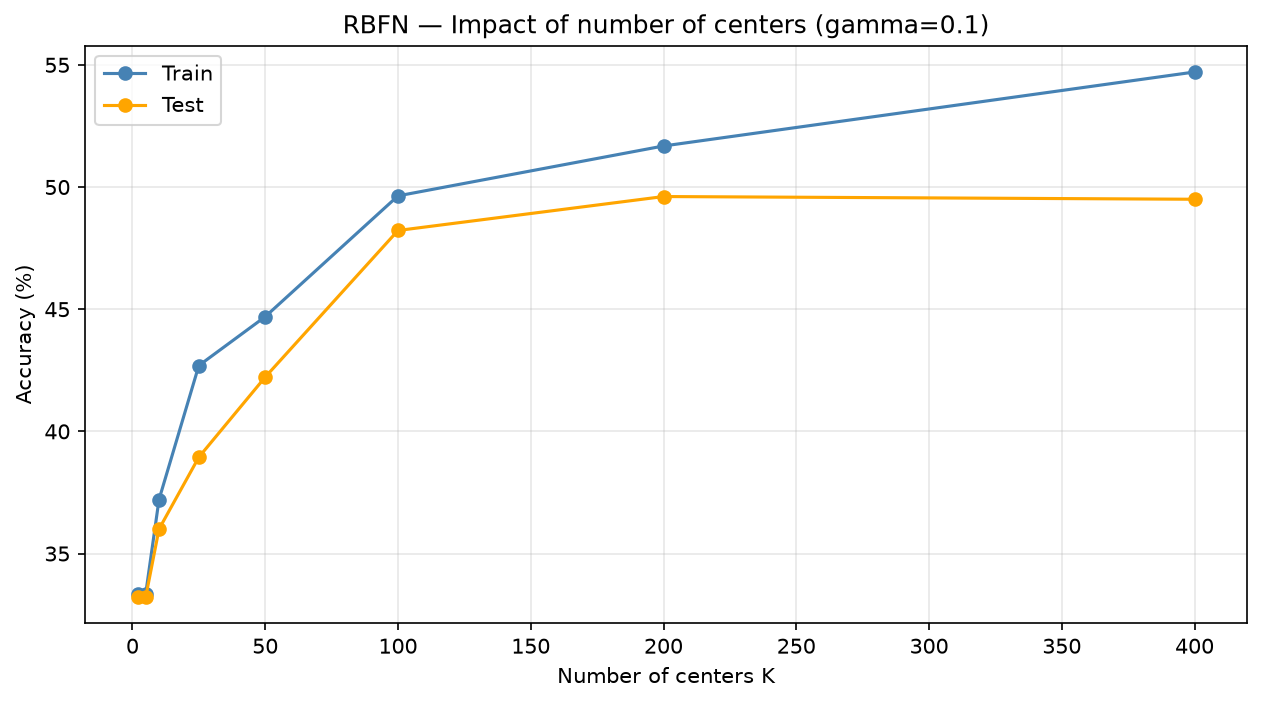
\includegraphics[width=0.85\linewidth]{report_plots/rbfn_k_sweep.png}
\caption{RBFN --- Influence du nombre de centres}
\end{figure}

\hypertarget{expuxe9rience-3-version-nauxefve-contre-k-centres}{%
\section{Expérience 3 --- Version naïve contre K
centres}\label{expuxe9rience-3-version-nauxefve-contre-k-centres}}

Cette expérience oppose directement les deux approches sur un jeu réduit
à cent exemples par classe, la version naïve nécessitant l'inversion
d'une matrice dont la taille est celle du nombre d'exemples. Le résultat
est la démonstration la plus nette de tout notre travail sur le RBFN. La
version naïve, qui garde chaque exemple comme centre, atteint cent pour
cent en apprentissage mais seulement quarante pour cent en test. Elle
classe donc parfaitement les exemples qu'elle a vus, puisque chacun se
trouve exactement sur son propre centre, mais généralise mal.

La version à trente centres obtient quant à elle cinquante-trois pour
cent en apprentissage et trente-huit pour cent en test. Elle apprend
donc moins bien les exemples d'entraînement, précisément parce qu'elle
ne les mémorise pas. Cet écart de soixante points entre l'apprentissage
à cent pour cent de la version naïve et sa piètre performance en test
est l'illustration parfaite du principe énoncé en conclusion du cours :
généraliser n'est pas minimiser l'erreur sur les exemples. Un modèle qui
possède autant de paramètres que d'exemples peut toujours mémoriser
parfaitement son jeu d'apprentissage, ce qui n'est en rien une garantie
de bonne généralisation.

\begin{figure}[htbp]
\centering
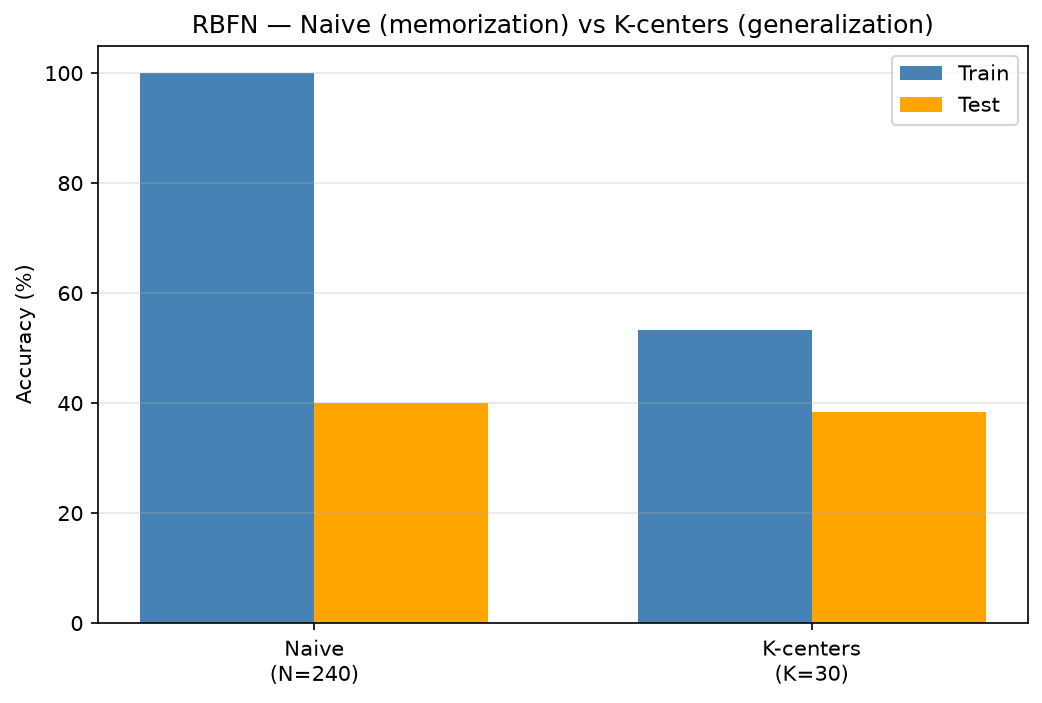
\includegraphics[width=0.85\linewidth]{report_plots/rbfn_naive_vs_kcenters.png}
\caption{RBFN --- Version naïve contre K centres}
\end{figure}

\hypertarget{expuxe9rience-4-matrice-de-confusion-1}{%
\section{Expérience 4 --- Matrice de
confusion}\label{expuxe9rience-4-matrice-de-confusion-1}}

Nous avons enfin examiné la matrice de confusion du réseau à cinquante
centres. La précision globale s'établit autour de quarante-deux pour
cent, avec une fois encore de fortes disparités entre classes. Dans
cette configuration, le guépard devient la classe la mieux reconnue,
avec près de soixante-quinze pour cent de bonnes classifications, tandis
que le lion devient la plus faible, à environ dix-sept pour cent.

Ce profil d'erreur est particulièrement instructif lorsqu'on le
rapproche de nos autres modèles. Le RBFN sur caractéristiques extraites
échouait sur le guépard, le perceptron sur pixels bruts échouait sur le
lion, et le RBFN sur pixels bruts échoue lui aussi sur le lion tout en
réussissant le guépard. Chaque combinaison de modèle et de
représentation échoue donc sur une classe différente. Cette observation,
cohérente avec ce que nous avions déjà constaté pour le perceptron,
confirme que le choix du modèle et de la représentation ne déplace pas
seulement la précision globale mais détermine sur quelle classe le
système se trompe.

\begin{figure}[htbp]
\centering
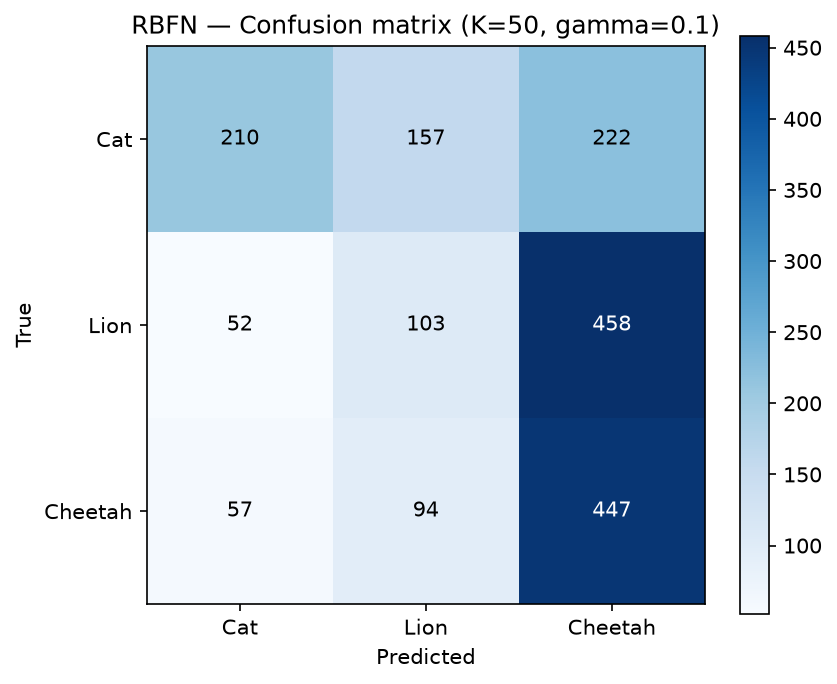
\includegraphics[width=0.85\linewidth]{report_plots/rbfn_confusion.png}
\caption{RBFN --- Matrice de confusion}
\end{figure}

\hypertarget{synthuxe8se-2}{%
\section{Synthèse}\label{synthuxe8se-2}}

L'étude du RBFN met en évidence, sur un modèle de nature très différente
du perceptron, les mêmes phénomènes fondamentaux. Le paramètre gamma
révèle un arbitrage clair entre cloches trop larges qui sous-apprennent
et cloches trop étroites qui mémorisent et s'effondrent. Le nombre de
centres montre qu'il en faut assez pour couvrir l'espace mais que trop
de centres finit par nuire à la généralisation. La comparaison entre
version naïve et version à K centres offre la démonstration la plus
limpide que mémoriser parfaitement l'apprentissage ne garantit nullement
la généralisation. Enfin, la nécessité d'une régularisation pour éviter
les matrices singulières en haute dimension constitue une limite
pratique importante du modèle, que le cours laisse entrevoir à travers
ses avertissements sur le choix de gamma. Comme pour le perceptron, la
performance plafonne à un niveau modeste qui tient moins au modèle
lui-même qu'à la difficulté de distinguer trois félins visuellement
proches, et le profil d'erreur par classe rappelle que représentation et
modèle façonnent ensemble ce que le système sait et ne sait pas faire.

\begin{center}\rule{0.5\linewidth}{0.5pt}\end{center}

\hypertarget{uxe9tude-expuxe9rimentale-du-support-vector-machine}{%
\chapter{Étude expérimentale du Support Vector
Machine}\label{uxe9tude-expuxe9rimentale-du-support-vector-machine}}

\hypertarget{cadre-muxe9thodologique-3}{%
\section{Cadre méthodologique}\label{cadre-muxe9thodologique-3}}

Le Support Vector Machine repose sur une idée différente des modèles
précédents : parmi toutes les frontières qui séparent deux classes, il
cherche celle dont la marge, c'est-à-dire le couloir vide de part et
d'autre de la frontière, est la plus large possible. Cette frontière
optimale n'est déterminée que par une poignée de points, ceux qui
touchent le bord du couloir, appelés vecteurs supports. Tous les autres
points n'ont aucune influence, ce qui fait du SVM un modèle
intrinsèquement parcimonieux au sens de la préférence pour la simplicité
que le cours défend.

Le SVM étant fondamentalement un classifieur binaire, nous l'appliquons
à nos trois classes selon la stratégie un-contre-tous, exactement comme
pour le perceptron de Rosenblatt : nous entraînons un classifieur par
classe, puis nous retenons pour chaque exemple la classe dont la valeur
de décision est la plus élevée. Pour traiter les données non
linéairement séparables, nous utilisons l'astuce du noyau, qui remplace
le produit scalaire par une fonction de similarité. Nous comparons le
noyau linéaire au noyau RBF, ce dernier étant la même gaussienne que
celle de notre RBFN.

Deux points pratiques ont guidé l'implémentation. D'abord, la résolution
du programme quadratique dual est confiée à la bibliothèque OSQP, qui
procède par éclatement d'opérateurs : elle alterne entre une résolution
linéaire tenant compte de la contrainte d'égalité et une simple
projection qui ramène les coefficients négatifs à zéro, jusqu'à
convergence. Ensuite, un SVM à marge dure suppose que les données sont
parfaitement séparables, ce qui n'est jamais le cas de données réelles ;
nous avons donc ajouté la marge souple, contrôlée par un paramètre C qui
borne l'influence maximale de chaque point et autorise ainsi quelques
violations de la marge en échange d'une frontière plus lisse.

Les résultats présentés utilisent la représentation par pixels bruts.
Comme pour la RBFN, cette représentation en grande dimension n'est pas
idéale pour une méthode à noyau, et nous verrons que le SVM y devient
extrêmement sensible au choix de gamma. En raison du coût de résolution
du programme quadratique, dense et de taille égale au nombre d'exemples
pour chacun des trois classifieurs un-contre-tous, nous entraînons le
SVM sur un sous-échantillon plus modeste que les autres modèles.

\hypertarget{expuxe9rience-1-influence-de-gamma-1}{%
\section{Expérience 1 --- Influence de
gamma}\label{expuxe9rience-1-influence-de-gamma-1}}

Cette expérience produit la courbe de sur-apprentissage la plus nette de
tout notre travail. À gamma faible, entre 0,001 et 0,01, le modèle
atteint environ soixante-quatorze à quatre-vingt-quatorze pour cent en
apprentissage et se maintient autour de cinquante-deux pour cent en test
: un modèle exploitable. Mais à mesure que gamma augmente, la précision
d'apprentissage grimpe inexorablement jusqu'à cent pour cent, tandis que
la précision de test s'effondre : quarante-deux pour cent à gamma égal à
0,05, trente-cinq pour cent à 0,1, puis le plancher de trente et un pour
cent, qui correspond à un modèle prédisant systématiquement une seule
classe.

Le mécanisme est exactement celui de la mémorisation extrême. Avec des
cloches gaussiennes trop étroites en grande dimension, chaque vecteur
support n'influence plus que lui-même, si bien que le modèle classe
parfaitement ses exemples d'apprentissage mais n'a plus rien à dire sur
un point de test. La leçon pratique est claire et constitue le principal
enseignement de notre étude du SVM : sur cette représentation, gamma est
un paramètre dangereux, dont une valeur à peine trop grande suffit à
faire basculer le modèle de l'apprentissage utile à la mémorisation
stérile.

\begin{figure}[htbp]
\centering
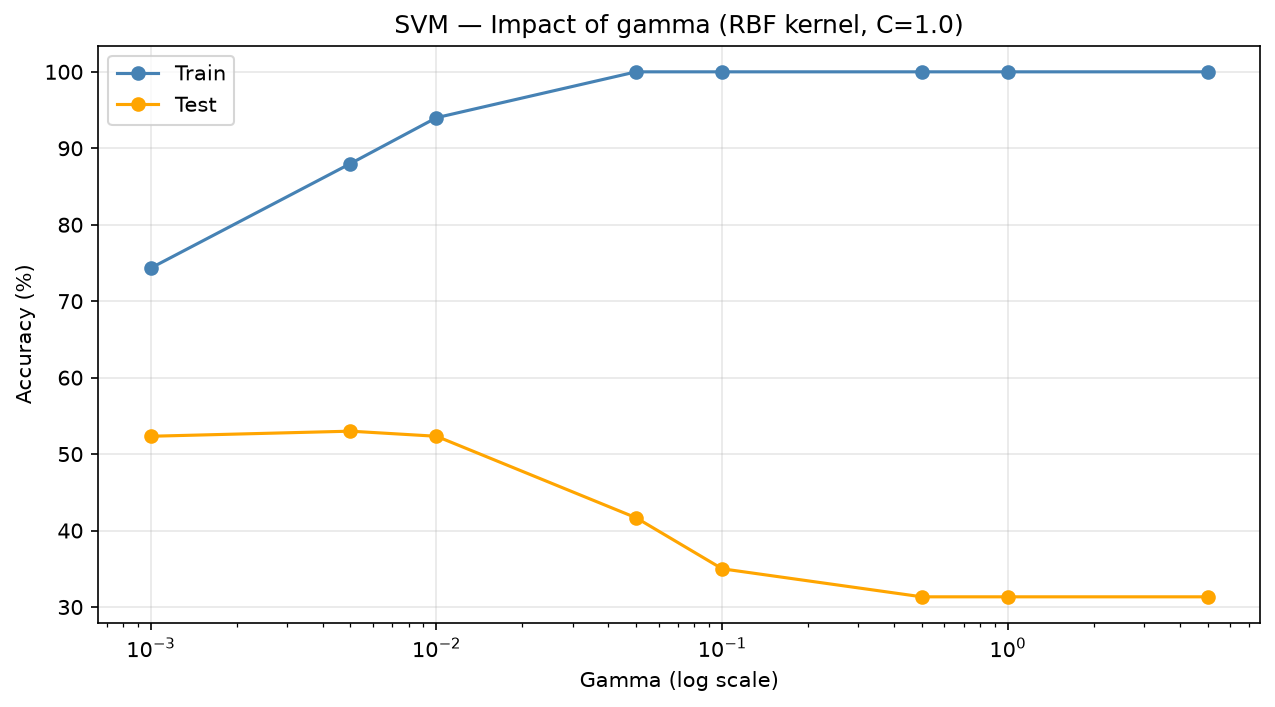
\includegraphics[width=0.85\linewidth]{report_plots/svm_gamma_sweep.png}
\caption{SVM --- Influence de gamma}
\end{figure}

\hypertarget{expuxe9rience-2-influence-de-c}{%
\section{Expérience 2 --- Influence de
C}\label{expuxe9rience-2-influence-de-c}}

Le paramètre C de la marge souple se comporte de façon plus douce que
gamma. À gamma fixé à une valeur raisonnable, augmenter C fait monter la
précision d'apprentissage vers cent pour cent, tandis que la précision
de test progresse d'environ quarante-sept pour cent jusqu'à
cinquante-quatre pour cent puis se stabilise. Contrairement à gamma,
augmenter C n'entraîne donc pas d'effondrement : parce que le noyau
n'est ici pas assez pointu pour mémoriser de façon destructrice,
resserrer la marge en augmentant C aide réellement la généralisation
jusqu'à un palier.

Ce contraste entre les deux paramètres est instructif. C règle la
tolérance aux violations de la marge, un arbitrage relativement stable,
alors que gamma règle la forme même de la frontière et peut la rendre
arbitrairement contournée. Le comportement observé confirme que, sur nos
données, le risque de sur-apprentissage provient bien davantage de gamma
que de C.

\begin{figure}[htbp]
\centering
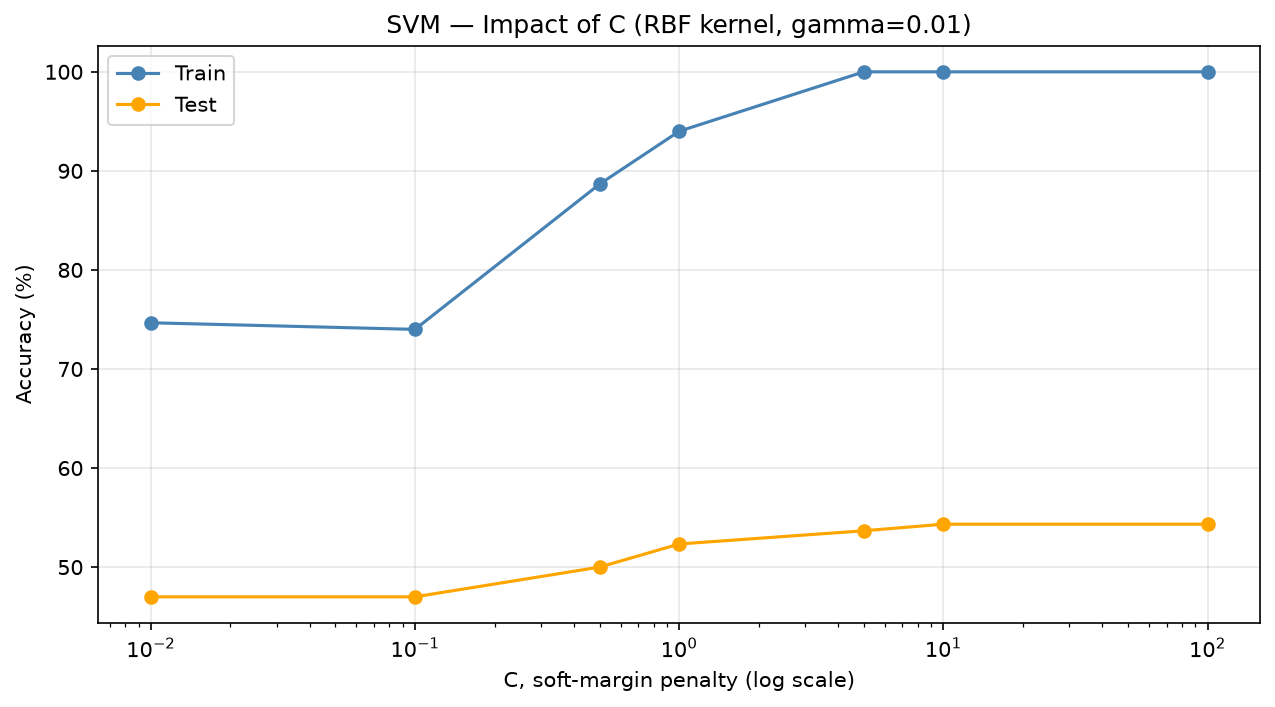
\includegraphics[width=0.85\linewidth]{report_plots/svm_c_sweep.png}
\caption{SVM --- Influence de C}
\end{figure}

\hypertarget{expuxe9rience-3-interaction-gamma-et-c}{%
\section{Expérience 3 --- Interaction gamma et
C}\label{expuxe9rience-3-interaction-gamma-et-c}}

Comme les deux paramètres agissent conjointement, nous avons balayé une
grille de valeurs et représenté la précision de test sous forme de carte
de chaleur. Elle rend l'interaction immédiatement lisible. Toute la
bande à gamma élevé, à partir de 0,1, est effondrée entre trente et un
et trente-sept pour cent, quelle que soit la valeur de C : une fois
gamma trop grand, aucun réglage de C ne peut rattraper la frontière. La
performance exploitable vit entièrement dans la bande à gamma faible, où
le meilleur compromis se situe à gamma égal à 0,01 et C égal à 10, pour
cinquante-quatre virgule trois pour cent en test.

Cette figure résume à elle seule la stratégie de réglage du SVM sur ce
problème : choisir d'abord un gamma suffisamment faible pour éviter
l'effondrement, puis n'utiliser C que comme un réglage fin.

\begin{figure}[htbp]
\centering
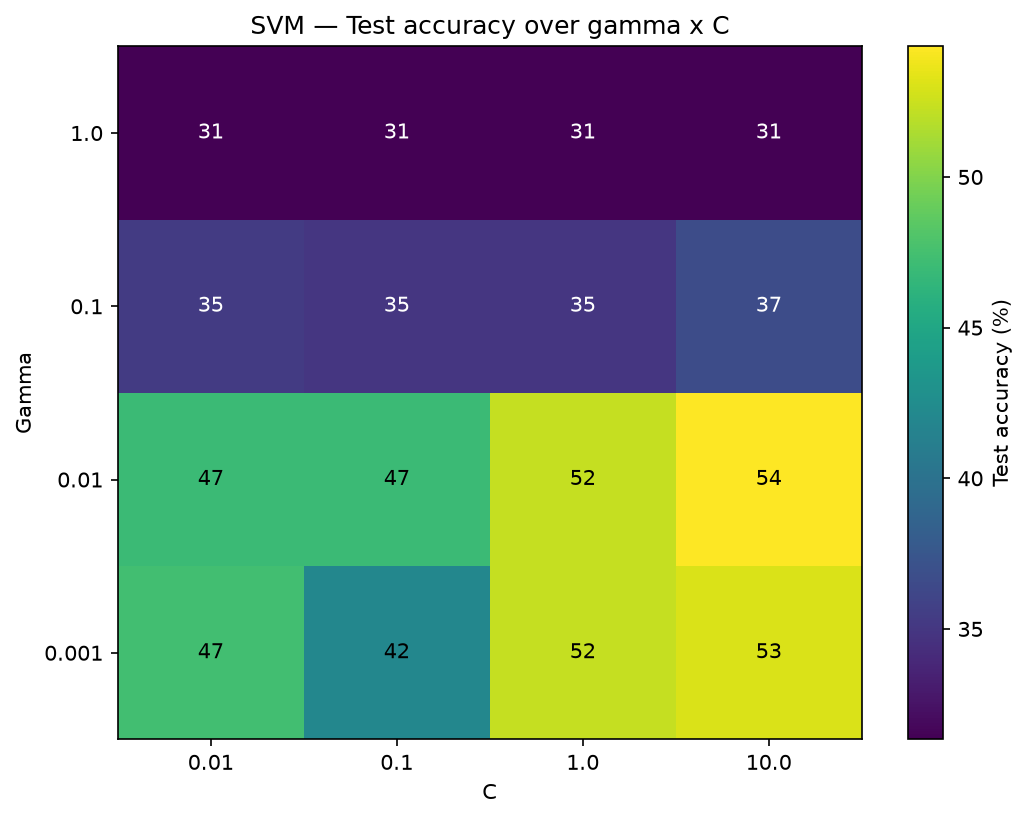
\includegraphics[width=0.85\linewidth]{report_plots/svm_gamma_c_heatmap.png}
\caption{SVM --- Carte de chaleur gamma et C}
\end{figure}

\hypertarget{expuxe9rience-4-noyau-linuxe9aire-contre-noyau-rbf}{%
\section{Expérience 4 --- Noyau linéaire contre noyau
RBF}\label{expuxe9rience-4-noyau-linuxe9aire-contre-noyau-rbf}}

Nous avons comparé les deux noyaux sur les mêmes données. Le noyau RBF
l'emporte avec cinquante-deux pour cent en test contre quarante-quatre
pour cent pour le noyau linéaire. Le point remarquable est que le noyau
linéaire atteint cent pour cent en apprentissage tout en généralisant
moins bien : avec trois mille soixante-douze caractéristiques pour
seulement quelques centaines d'exemples d'apprentissage, même une
frontière linéaire dispose d'assez de liberté pour mémoriser
parfaitement le jeu d'apprentissage. Le noyau RBF, avec une frontière
plus lisse à gamma faible, généralise mieux malgré une précision
d'apprentissage plus basse.

Cette observation illustre concrètement que minimiser l'erreur sur les
exemples n'est pas généraliser : le noyau qui apprend le mieux ses
exemples n'est pas celui qui se comporte le mieux sur des données
nouvelles.

\begin{figure}[htbp]
\centering
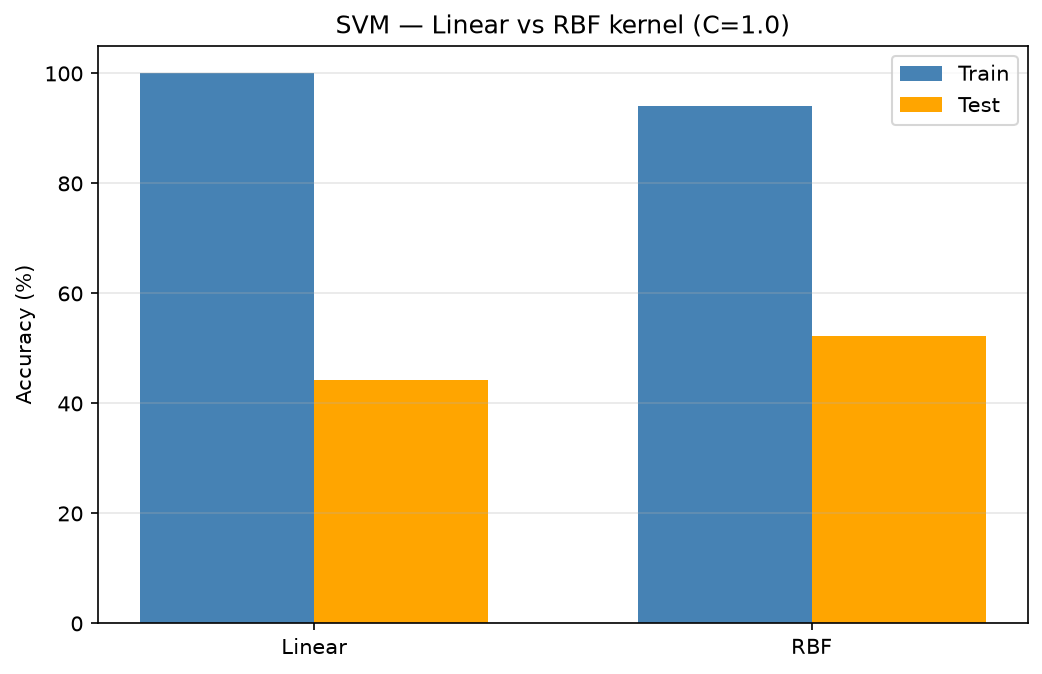
\includegraphics[width=0.85\linewidth]{report_plots/svm_linear_vs_rbf.png}
\caption{SVM --- Noyau linéaire contre RBF}
\end{figure}

\hypertarget{expuxe9rience-5-matrice-de-confusion}{%
\section{Expérience 5 --- Matrice de
confusion}\label{expuxe9rience-5-matrice-de-confusion}}

Nous avons enfin examiné la matrice de confusion au meilleur réglage
identifié par la carte de chaleur, gamma égal à 0,01 et C égal à 10. La
précision globale s'établit à cinquante-quatre virgule trois pour cent,
et surtout les trois classes sont désormais réellement prédites, sans
l'effondrement vers une seule classe que produisaient les mauvais
réglages. Le chat est la classe la mieux reconnue à environ
soixante-seize pour cent, le lion se situe à cinquante pour cent, et le
guépard reste le plus difficile à trente-neuf pour cent.

Ce profil, où le guépard est la classe la plus faible, rejoint ce que
nous avons constaté pour tous nos modèles : la confusion entre lion et
guépard demeure la source d'erreur principale, quelle que soit
l'approche employée. Le SVM ne fait pas exception à ce constat
transversal.

\begin{figure}[htbp]
\centering
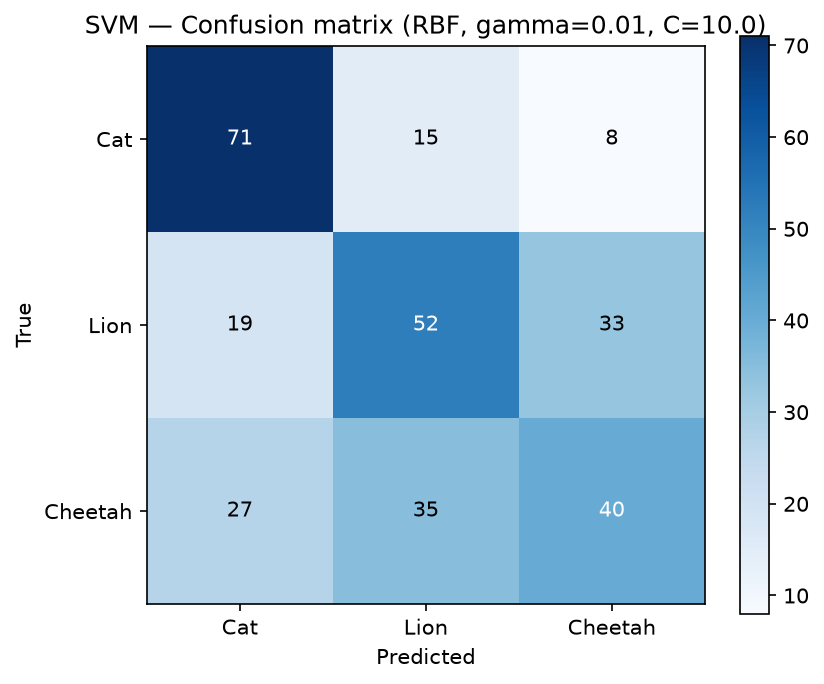
\includegraphics[width=0.85\linewidth]{report_plots/svm_confusion.png}
\caption{SVM --- Matrice de confusion}
\end{figure}

\hypertarget{synthuxe8se-3}{%
\section{Synthèse}\label{synthuxe8se-3}}

L'étude du SVM confirme, sur un modèle de nature encore différente, les
phénomènes récurrents de tout le projet. Le paramètre gamma révèle un
arbitrage brutal entre frontière trop lisse et mémorisation, et se
montre bien plus dangereux que le paramètre C de la marge souple, plus
stable. Le noyau RBF surpasse le noyau linéaire tout en apprenant moins
parfaitement ses exemples, illustration directe de la différence entre
apprentissage et généralisation. La nécessité de la marge souple pour
traiter des données réelles non séparables constitue une limite pratique
importante du modèle idéal des diapositives, et l'extrême sensibilité à
gamma sur les pixels bruts montre qu'une méthode à noyau n'est pas la
mieux adaptée à une représentation de si grande dimension : une
représentation plus compacte, ou une réduction de dimension préalable,
servirait mieux ce modèle. Comme pour les autres approches, la
performance finale, autour de cinquante-quatre pour cent, se heurte
moins aux limites du SVM lui-même qu'à la difficulté intrinsèque de
distinguer trois félins visuellement proches, et le profil d'erreur par
classe demeure celui de tous nos modèles.

\begin{center}\rule{0.5\linewidth}{0.5pt}\end{center}

\hypertarget{comparaison-transversale-des-moduxe8les}{%
\chapter{Comparaison transversale des
modèles}\label{comparaison-transversale-des-moduxe8les}}

\hypertarget{performances-finales}{%
\section{Performances finales}\label{performances-finales}}

Le tableau suivant récapitule les meilleures configurations observées
pour chaque modèle sur le jeu de données réel, avec la représentation
utilisée pour chaque mesure.

\begin{longtable}[]{@{}
  >{\raggedright\arraybackslash}p{(\columnwidth - 6\tabcolsep) * \real{0.2500}}
  >{\raggedright\arraybackslash}p{(\columnwidth - 6\tabcolsep) * \real{0.2500}}
  >{\raggedright\arraybackslash}p{(\columnwidth - 6\tabcolsep) * \real{0.2500}}
  >{\raggedright\arraybackslash}p{(\columnwidth - 6\tabcolsep) * \real{0.2500}}@{}}
\toprule\noalign{}
\begin{minipage}[b]{\linewidth}\raggedright
Modèle
\end{minipage} & \begin{minipage}[b]{\linewidth}\raggedright
Représentation
\end{minipage} & \begin{minipage}[b]{\linewidth}\raggedright
Apprentissage
\end{minipage} & \begin{minipage}[b]{\linewidth}\raggedright
Test
\end{minipage} \\
\midrule\noalign{}
\endhead
\bottomrule\noalign{}
\endlastfoot
Rosenblatt & extract, vingt caractéristiques & environ quarante-sept
pour cent & environ quarante-deux pour cent \\
MLP & extract, vingt caractéristiques & environ soixante-six pour cent &
environ cinquante-six pour cent \\
RBFN & flatten, meilleure configuration & environ cinquante-six pour
cent & environ cinquante-quatre pour cent \\
SVM & flatten, gamma 0,01 et C 10 & cent pour cent & cinquante-quatre
virgule trois pour cent \\
\end{longtable}

La hiérarchie observée est cohérente avec la complexité des modèles. Le
perceptron linéaire, incapable de tracer autre chose qu'un hyperplan,
plafonne le plus bas et converge même vers une solution dégénérée qui
prédit majoritairement une seule classe. Le MLP domine grâce à ses
couches cachées non linéaires. Le RBFN et le SVM, tous deux fondés sur
la même gaussienne, atteignent des niveaux comparables lorsque leurs
hyperparamètres sont correctement réglés, mais au prix d'une sensibilité
bien plus grande à ces réglages.

\hypertarget{le-profil-des-erreurs-comme-signature-du-couple-moduxe8le-repruxe9sentation}{%
\section{Le profil des erreurs comme signature du couple
modèle-représentation}\label{le-profil-des-erreurs-comme-signature-du-couple-moduxe8le-repruxe9sentation}}

L'observation la plus riche de tout le projet ne porte pas sur les
précisions globales mais sur les matrices de confusion. Chaque
combinaison d'un modèle et d'une représentation échoue sur une classe
différente. Le MLP sur caractéristiques extraites confond massivement le
lion avec le guépard. Le MLP sur pixels bruts inverse le problème et
confond le lion avec le chat. Le RBFN sur caractéristiques extraites
écrase le guépard, tandis que le RBFN sur pixels bruts réussit le
guépard et échoue sur le lion. Le SVM au meilleur réglage reconnaît bien
le chat et reste faible sur le guépard. Le perceptron, lui, s'effondre
entièrement vers le lion.

Autrement dit, aucune approche n'est uniformément supérieure : la
représentation d'entrée et le modèle façonnent ensemble non seulement le
niveau de performance mais la nature même des erreurs. Les
caractéristiques extraites capturent la couleur et la texture globales,
et distinguent donc bien les classes qui diffèrent par ces attributs ;
les pixels bruts conservent une information spatiale diffuse qu'un
modèle assez capable exploite différemment. La confusion entre lion et
guépard, récurrente sous toutes les approches, s'explique visuellement
sans peine : fourrure fauve, morphologie proche, décor de savane
similaire ; aucun de nos descripteurs ne capture ce qui les distingue
vraiment, la crinière, les motifs du pelage ou la silhouette.

\hypertarget{couxfbt-et-nature-de-lentrauxeenement}{%
\section{Coût et nature de
l'entraînement}\label{couxfbt-et-nature-de-lentrauxeenement}}

Les quatre modèles diffèrent aussi profondément par leur procédure
d'entraînement. Le perceptron et le MLP apprennent par itérations
successives, avec un coût proportionnel au nombre d'époques et
d'exemples ; le MLP journalise ainsi naturellement des courbes
d'apprentissage. Le RBFN s'entraîne en un seul coup, un k-means suivi
d'une pseudo-inverse, ce qui le rend très rapide sur les
caractéristiques extraites mais coûteux quand la matrice grandit. Le SVM
résout un programme quadratique dense dont la taille est le carré du
nombre d'exemples, et ce trois fois pour la stratégie un-contre-tous :
c'est le modèle le plus coûteux à entraîner à grande échelle, ce qui
nous a conduits à limiter la taille de son jeu d'apprentissage, tout en
l'évaluant sur un jeu de test large pour que ses chiffres restent
comparables.

\begin{center}\rule{0.5\linewidth}{0.5pt}\end{center}

\hypertarget{difficultuxe9s-rencontruxe9es-et-ruxe9solutions}{%
\chapter{Difficultés rencontrées et
résolutions}\label{difficultuxe9s-rencontruxe9es-et-ruxe9solutions}}

Ce chapitre rassemble les problèmes réels rencontrés au fil du projet et
la manière dont nous les avons diagnostiqués puis résolus. Nous les
présentons dans l'ordre à peu près chronologique du projet, car
plusieurs résolutions ont directement nourri la suite du travail.

\hypertarget{le-ruxe9seau-qui-refusait-dapprendre}{%
\section{Le réseau qui refusait
d'apprendre}\label{le-ruxe9seau-qui-refusait-dapprendre}}

Le tout premier entraînement du MLP est resté figé à exactement
trente-trois virgule trois pour cent pendant cinq mille époques, le
niveau du hasard pour trois classes, avec une perte quasiment immobile.
Le coupable était l'initialisation des poids : notre code multipliait
une plage aléatoire déjà minuscule, entre moins zéro virgule zéro un et
zéro virgule zéro un, par le facteur de He, produisant des poids si
proches de zéro que toutes les sorties étaient identiques et que les
gradients s'évanouissaient avant de pouvoir modifier quoi que ce soit.
La correction a consisté à tirer les poids dans la plage entre moins un
et un et à laisser le facteur de He assurer seul la mise à l'échelle.
L'apprentissage a fonctionné immédiatement après, avec cent pour cent de
réussite sur les points synthétiques. La leçon retenue : un réseau
bloqué exactement au niveau du hasard doit faire suspecter
l'initialisation avant l'algorithme.

\hypertarget{lordre-des-opuxe9rations-dans-la-ruxe9tropropagation}{%
\section{L'ordre des opérations dans la
rétropropagation}\label{lordre-des-opuxe9rations-dans-la-ruxe9tropropagation}}

Sur données réelles, le programme s'est ensuite interrompu sur une
incompatibilité de dimensions dans une soustraction de matrices. La
cause était l'ordre des opérations dans la boucle de rétropropagation :
nous calculions le delta de la couche précédente avant d'avoir mis à
jour les poids de la couche courante, si bien qu'au moment d'utiliser le
delta pour le gradient de la couche courante, il avait déjà été écrasé
par un delta de la mauvaise dimension. Inverser les deux étapes, mettre
à jour d'abord, transformer le delta ensuite, a réglé le problème. Cette
erreur nous a fait réellement intérioriser l'ordonnancement canonique de
la rétropropagation, que nous avions lu sans le comprendre en
profondeur.

\hypertarget{le-module-fantuxf4me}{%
\section{Le module fantôme}\label{le-module-fantuxf4me}}

Après avoir écrit les premiers fichiers du RBFN avec leurs tests, la
commande de test n'exécutait aucun test du module : le compilateur les
ignorait purement et simplement, car les déclarations de module
n'avaient pas été ajoutées, ni dans le module rbfn lui-même ni dans la
liste des modèles. Deux lignes de déclaration ont suffi. L'enseignement
est propre à Rust : un fichier non déclaré n'existe pas pour le
compilateur, et l'absence de tests dans la sortie doit y faire penser
immédiatement.

\hypertarget{le-bug-daccumulation-duxe9tectuxe9-par-les-tests}{%
\section{Le bug d'accumulation détecté par les
tests}\label{le-bug-daccumulation-duxe9tectuxe9-par-les-tests}}

Un test du RBFN calculant la distance au carré entre les points
zéro-zéro et trois-quatre attendait vingt-cinq et obtenait seize. La
boucle d'accumulation écrasait la somme à chaque itération au lieu d'y
ajouter la contribution de chaque dimension, un simple signe égal là où
il fallait un plus-égal. Le point remarquable est que le test de
distance nulle passait, lui, sans problème : quand toutes les
contributions valent zéro, écraser ou accumuler donne le même résultat.
Il a fallu un cas à deux dimensions non nulles pour exposer le bug.
C'est l'illustration la plus nette de la valeur de nos tests unitaires :
une erreur d'un caractère, invisible sur les cas simples, aurait
silencieusement faussé toutes les distances du RBFN et du noyau RBF du
SVM, qui réutilise la même fonction.

\hypertarget{les-matrices-singuliuxe8res-en-haute-dimension}{%
\section{Les matrices singulières en haute
dimension}\label{les-matrices-singuliuxe8res-en-haute-dimension}}

Lors du balayage de gamma du RBFN en pixels bruts, le programme a
paniqué en pleine expérience : matrice singulière, impossible à
inverser. En trois mille soixante-douze dimensions, de nombreuses
colonnes de la matrice Phi deviennent presque identiques, le déterminant
s'effondre et l'élimination de Gauss-Jordan rencontre un pivot nul. La
solution standard, la régularisation de type ridge, ajoute une valeur
minuscule sur la diagonale avant l'inversion, ce qui garantit
l'inversibilité sans altérer sensiblement la solution. Nous avons
ensuite réutilisé exactement la même idée dans le SVM, où une petite
crête sur la diagonale de la matrice Q garantit la semi-définie
positivité numérique que le solveur exige. Cette difficulté purement
numérique, absente des diapositives, est un bon exemple de l'écart entre
les mathématiques idéales et leur mise en œuvre en virgule flottante.

\hypertarget{la-compilation-dosqp}{%
\section{La compilation d'OSQP}\label{la-compilation-dosqp}}

L'ajout de la dépendance OSQP pour le SVM a échoué dès la compilation :
le projet C embarqué par la crate déclare une version minimale de CMake
si ancienne que les CMake modernes refusent de la traiter. La solution
documentée par CMake lui-même consiste à définir la variable
d'environnement autorisant les anciennes politiques, après quoi la
compilation aboutit. Ce genre d'incident illustre le coût caché des
dépendances natives : la crate est correcte, mais son environnement de
compilation vieillit indépendamment d'elle.

\hypertarget{linfaisabilituxe9-de-la-marge-dure}{%
\section{L'infaisabilité de la marge
dure}\label{linfaisabilituxe9-de-la-marge-dure}}

Le premier lancement du SVM sur le jeu synthétique non linéairement
séparable a fait paniquer le programme : le solveur ne trouvait aucune
solution. Ce n'était pas un bug mais un fait mathématique : notre SVM
était alors à marge dure, il suppose qu'un hyperplan séparateur existe,
et sur des classes entrelacées avec un noyau linéaire il n'en existe
aucun, si bien que le problème d'optimisation n'a pas de solution
réalisable. Le solveur, correctement, le signale plutôt que de renvoyer
un résultat absurde. Nous avons d'abord contourné en ne démontrant que
le noyau RBF sur les cas synthétiques, en sachant expliquer pourquoi le
noyau linéaire échouerait, puis traité la cause en profondeur avec la
marge souple.

\hypertarget{leffondrement-par-muxe9morisation-du-svm}{%
\section{L'effondrement par mémorisation du
SVM}\label{leffondrement-par-muxe9morisation-du-svm}}

Entraîné sur les sept mille deux cents exemples complets, le SVM a
produit le résultat le plus spectaculairement pathologique du projet :
cent pour cent en apprentissage, trente-trois virgule neuf pour cent en
test, et une matrice de confusion où la quasi-totalité des mille huit
cents images de test était prédite lion. Le diagnostic croise deux
causes. D'une part, la marge dure n'offre aucune défense contre le
sur-apprentissage : elle exige une séparation parfaite, aussi contournée
soit la frontière. D'autre part, en très haute dimension, quelques
centaines de points sont presque toujours parfaitement séparables, donc
le modèle peut toujours mémoriser. Nous avons répondu sur trois fronts :
l'ajout de la marge souple, qui borne l'influence de chaque point par le
paramètre C et se réduit à changer la borne supérieure des coefficients
dans le programme quadratique ; la réduction du jeu d'apprentissage du
SVM, évalué en revanche sur un jeu de test large ; et le réglage
conjoint de gamma et de C, dont la carte de chaleur du chapitre huit
montre le résultat. Même après ces corrections, un premier essai en
pixels bruts à C très faible restait effondré, confirmant que dans cette
configuration le paramètre décisif était gamma et non C, ce que la carte
de chaleur a ensuite établi proprement.

\hypertarget{la-matrice-de-confusion-du-mauvais-ruxe9glage}{%
\section{La matrice de confusion du mauvais
réglage}\label{la-matrice-de-confusion-du-mauvais-ruxe9glage}}

Une subtilité de nos propres scripts d'expérimentation a failli fausser
le rapport : l'expérience de la matrice de confusion utilisait des
valeurs de gamma et de C codées en dur, qui se sont avérées être
précisément une configuration effondrée. La matrice montrait donc le
pire modèle en le présentant comme le meilleur. La correction a consisté
à faire retourner par l'expérience de la carte de chaleur sa meilleure
configuration, et à la transmettre à l'expérience de la matrice de
confusion, qui reflète désormais toujours le véritable optimum du
balayage. La leçon dépasse le cas d'espèce : dans une chaîne
d'expériences, les constantes codées en dur deviennent fausses dès que
les expériences amont évoluent.

\hypertarget{les-pertes-de-code-lors-des-fusions}{%
\section{Les pertes de code lors des
fusions}\label{les-pertes-de-code-lors-des-fusions}}

Le travail à deux sur un même dépôt a produit son lot classique
d'accidents de fusion. À deux reprises, des blocs entiers de nos
exécutables de test se sont retrouvés commentés ou supprimés après une
fusion, sans erreur de compilation puisque le code restant était valide.
Le symptôme révélateur était ailleurs : une pluie d'avertissements sur
des imports et des variables inutilisés. Plutôt que de faire taire ces
avertissements, nous les avons traités comme un signal : si les
variables du découpage apprentissage-test sont inutilisées, c'est que le
code qui les consommait a disparu. La restauration s'est faite depuis
l'historique, et nous en avons profité pour consolider les fichiers de
test, en fusionnant notamment les jeux de données synthétiques dupliqués
entre les sections des différents modèles. Un avertissement de
compilation après une fusion n'est pas du bruit : c'est souvent la seule
trace d'un travail perdu.

\hypertarget{le-carnet-de-tests-uxe9vaporuxe9-et-sa-ruxe9cupuxe9ration}{%
\section{Le carnet de tests évaporé et sa
récupération}\label{le-carnet-de-tests-uxe9vaporuxe9-et-sa-ruxe9cupuxe9ration}}

Peu avant l'assemblage du rapport, le carnet Jupyter des cas de tests
s'est retrouvé vide, et son point de contrôle automatique l'était aussi.
La récupération est passée par l'historique Git, mais sans savoir lequel
des trente-cinq commits contenait la bonne version. La méthode a
consisté à lister, pour chaque commit ayant touché un carnet, la taille
du fichier dans ce commit : les versions vides pèsent quelques
kilo-octets, les versions pleines de sorties graphiques plusieurs
centaines. La taille a immédiatement désigné le bon fichier, un carnet
de plus d'un mégaoctet contenant l'ensemble des démonstrations avec
leurs tracés de frontières de décision, restauré en une commande. Deux
leçons pratiques : la taille d'un fichier dans l'historique est un
critère de recherche redoutablement efficace, et il faut valider les
carnets dans le dépôt aussi souvent que le code.

\hypertarget{les-tests-du-duxe9coupage-stratifiuxe9}{%
\section{Les tests du découpage
stratifié}\label{les-tests-du-duxe9coupage-stratifiuxe9}}

La stratification du découpage apprentissage-test a elle-même cassé deux
tests existants, pour des raisons instructives. Le premier vérifiait la
taille exacte du jeu de test : or la stratification remplace un arrondi
global par la somme de trois arrondis par classe, qui peut différer de
quelques unités ; le test vérifie désormais la proximité et la
conservation du nombre total d'exemples. Le second vérifiait que deux
graines différentes produisent des découpages différents en comparant
les étiquettes : mais un découpage stratifié produit toujours la même
séquence d'étiquettes, classe par classe, quelle que soit la graine ;
seuls les exemples choisis changent. Le test compare désormais les
données elles-mêmes. Par ailleurs, la première dérivation de graine par
classe, une simple addition, créait des collisions entre graines
globales voisines ; la dérivation par multiplication par un grand nombre
impair les a éliminées. Ces trois corrections illustrent qu'un
changement d'algorithme correct peut invalider des tests qui encodaient,
sans le dire, des propriétés de l'ancienne implémentation.

\begin{center}\rule{0.5\linewidth}{0.5pt}\end{center}

\hypertarget{interface-et-livrables}{%
\chapter{Interface et livrables}\label{interface-et-livrables}}

L'interface graphique, construite avec Gradio, est organisée en trois
onglets. L'onglet de classification permet de téléverser une image, de
choisir le modèle parmi les quatre, et d'obtenir la prédiction ; le
prétraitement appliqué à l'image est automatiquement celui avec lequel
le modèle sélectionné a été entraîné, grâce aux métadonnées
sauvegardées. Pour le MLP, les sorties brutes sont converties en
pseudo-probabilités par une fonction softmax appliquée en aval,
présentation plus lisible qu'une normalisation min-max qui affichait
trompeusement cent pour cent et zéro pour cent ; nous savons expliquer
que ces valeurs, le réseau n'ayant pas été entraîné avec une sortie
softmax, sont un affichage de confiance relative et non des probabilités
calibrées.

L'onglet d'entraînement propose un sous-onglet par modèle, chacun
exposant ses hyperparamètres propres : architecture, époques et taux
d'apprentissage pour le MLP ; nombre de centres, gamma et itérations de
k-means pour le RBFN ; époques, taux et graine pour le Rosenblatt ;
noyau, gamma, C et taille d'échantillon pour le SVM, dont le curseur de
taille est volontairement borné bas en raison du coût du programme
quadratique. Chaque entraînement effectue un découpage quatre-vingts
vingt, affiche les précisions d'apprentissage et de test, et sauvegarde
le modèle avec ses métadonnées. L'onglet d'état, enfin, récapitule les
modèles disponibles et leurs réglages.

Les autres livrables sont l'exécutable de tests synthétiques, qui
déroule les quatre modèles sur un jeu linéairement séparable et un jeu
entrelacé non séparable, avec les cas d'échec du modèle linéaire et leur
résolution par transformation, par les couches cachées du MLP, par les
cloches du RBFN et par le noyau RBF du SVM ; l'exécutable de tests
réels, qui entraîne, évalue, affiche les matrices de confusion et
sauvegarde les quatre modèles sur le vrai jeu de données ; le carnet
Jupyter des cas de tests avec les tracés de frontières de décision ; et
les scripts Python d'expérimentation qui ont produit toutes les figures
de ce rapport.

\begin{center}\rule{0.5\linewidth}{0.5pt}\end{center}

\hypertarget{conclusion-et-perspectives}{%
\chapter{Conclusion et perspectives}\label{conclusion-et-perspectives}}

Au terme de ce projet, les quatre modèles exigés sont implémentés from
scratch en Rust, testés par plus de cent tests unitaires, exposés à
Python par une interface C, entraînables et utilisables depuis une
interface graphique, et étudiés expérimentalement en profondeur. Les
précisions finales, d'environ quarante-deux pour cent pour le perceptron
à cinquante-quatre à cinquante-six pour cent pour le MLP, le RBFN et le
SVM, peuvent sembler modestes dans l'absolu ; l'analyse montre qu'elles
tiennent moins aux modèles eux-mêmes qu'à la difficulté intrinsèque de
distinguer trois félins visuellement proches à partir de représentations
globales, la confusion entre lion et guépard traversant toutes nos
approches.

Les enseignements transversaux nous paraissent plus précieux que les
chiffres. Chaque modèle a rejoué, avec son propre vocabulaire, le même
arbitrage fondamental : époques et architecture pour le MLP, largeur des
cloches et nombre de centres pour le RBFN, gamma et C pour le SVM.
Partout, minimiser l'erreur sur les exemples s'est révélé distinct de
généraliser, avec pour démonstrations les plus frappantes la version
naïve du RBFN à cent pour cent d'apprentissage pour quarante pour cent
de test, et l'effondrement du SVM à marge dure. Partout aussi, la
représentation d'entrée s'est montrée au moins aussi déterminante que le
modèle, jusqu'à changer la classe sur laquelle le système échoue. Enfin,
l'écart entre les mathématiques idéales et leur implémentation, matrices
singulières, infaisabilités, initialisations dégénérées, a exigé des
réponses concrètes, régularisation, marge souple, tests unitaires, qui
font partie intégrante de ce que ce projet nous a appris.

Les perspectives d'amélioration découlent directement de l'analyse. Des
caractéristiques spatiales plus riches, capables de capturer la crinière
du lion ou les motifs du guépard, attaqueraient la confusion dominante
que nos vingt descripteurs globaux ne peuvent pas résoudre. Une
réduction de dimension préalable rendrait les pixels bruts exploitables
par les méthodes à noyau, qui s'y effondrent aujourd'hui. Un
entraînement multi-graines avec sélection du meilleur modèle
stabiliserait le perceptron. Et à plus long terme, des architectures
convolutives, hors du périmètre de ce projet, sont l'outil naturel de ce
type de problème, précisément parce qu'elles apprennent leurs propres
représentations au lieu de dépendre de descripteurs choisis à la main :
la conclusion rejoint ainsi la thèse centrale de ce rapport, la
performance d'un système d'apprentissage dépend au moins autant de la
représentation des données que du modèle qui les traite.


\end{document}
